%% Additional file 2 -- Guided installation and usage tutorial (GENERATED; do not edit).
%% Source: docs/tutorial.md. Rebuild: python submission/build_additional_file_2.py
%% Compiles standalone:  pdflatex additional_file_2_qsarena_tutorial
% Options for packages loaded elsewhere
\PassOptionsToPackage{unicode}{hyperref}
\PassOptionsToPackage{hyphens}{url}
\PassOptionsToPackage{dvipsnames,svgnames,x11names}{xcolor}
\documentclass[
  11pt,a4paper]{article}
\usepackage{xcolor}
\usepackage[margin=2cm]{geometry}
\usepackage{amsmath,amssymb}
\setcounter{secnumdepth}{-\maxdimen} % remove section numbering
\usepackage{iftex}
\ifPDFTeX
  \usepackage[T1]{fontenc}
  \usepackage[utf8]{inputenc}
  \usepackage{textcomp} % provide euro and other symbols
\else % if luatex or xetex
  \usepackage{unicode-math} % this also loads fontspec
  \defaultfontfeatures{Scale=MatchLowercase}
  \defaultfontfeatures[\rmfamily]{Ligatures=TeX,Scale=1}
\fi
\usepackage{lmodern}
\ifPDFTeX\else
  % xetex/luatex font selection
\fi
% Use upquote if available, for straight quotes in verbatim environments
\IfFileExists{upquote.sty}{\usepackage{upquote}}{}
\IfFileExists{microtype.sty}{% use microtype if available
  \usepackage[]{microtype}
  \UseMicrotypeSet[protrusion]{basicmath} % disable protrusion for tt fonts
}{}
\makeatletter
\@ifundefined{KOMAClassName}{% if non-KOMA class
  \IfFileExists{parskip.sty}{%
    \usepackage{parskip}
  }{% else
    \setlength{\parindent}{0pt}
    \setlength{\parskip}{6pt plus 2pt minus 1pt}}
}{% if KOMA class
  \KOMAoptions{parskip=half}}
\makeatother
\usepackage{color}
\usepackage{fancyvrb}
\newcommand{\VerbBar}{|}
\newcommand{\VERB}{\Verb[commandchars=\\\{\}]}
\DefineVerbatimEnvironment{Highlighting}{Verbatim}{commandchars=\\\{\}}
% Add ',fontsize=\small' for more characters per line
\usepackage{framed}
\definecolor{shadecolor}{RGB}{248,248,248}
\newenvironment{Shaded}{\begin{snugshade}}{\end{snugshade}}
\newcommand{\AlertTok}[1]{\textcolor[rgb]{0.94,0.16,0.16}{#1}}
\newcommand{\AnnotationTok}[1]{\textcolor[rgb]{0.56,0.35,0.01}{\textbf{\textit{#1}}}}
\newcommand{\AttributeTok}[1]{\textcolor[rgb]{0.13,0.29,0.53}{#1}}
\newcommand{\BaseNTok}[1]{\textcolor[rgb]{0.00,0.00,0.81}{#1}}
\newcommand{\BuiltInTok}[1]{#1}
\newcommand{\CharTok}[1]{\textcolor[rgb]{0.31,0.60,0.02}{#1}}
\newcommand{\CommentTok}[1]{\textcolor[rgb]{0.56,0.35,0.01}{\textit{#1}}}
\newcommand{\CommentVarTok}[1]{\textcolor[rgb]{0.56,0.35,0.01}{\textbf{\textit{#1}}}}
\newcommand{\ConstantTok}[1]{\textcolor[rgb]{0.56,0.35,0.01}{#1}}
\newcommand{\ControlFlowTok}[1]{\textcolor[rgb]{0.13,0.29,0.53}{\textbf{#1}}}
\newcommand{\DataTypeTok}[1]{\textcolor[rgb]{0.13,0.29,0.53}{#1}}
\newcommand{\DecValTok}[1]{\textcolor[rgb]{0.00,0.00,0.81}{#1}}
\newcommand{\DocumentationTok}[1]{\textcolor[rgb]{0.56,0.35,0.01}{\textbf{\textit{#1}}}}
\newcommand{\ErrorTok}[1]{\textcolor[rgb]{0.64,0.00,0.00}{\textbf{#1}}}
\newcommand{\ExtensionTok}[1]{#1}
\newcommand{\FloatTok}[1]{\textcolor[rgb]{0.00,0.00,0.81}{#1}}
\newcommand{\FunctionTok}[1]{\textcolor[rgb]{0.13,0.29,0.53}{\textbf{#1}}}
\newcommand{\ImportTok}[1]{#1}
\newcommand{\InformationTok}[1]{\textcolor[rgb]{0.56,0.35,0.01}{\textbf{\textit{#1}}}}
\newcommand{\KeywordTok}[1]{\textcolor[rgb]{0.13,0.29,0.53}{\textbf{#1}}}
\newcommand{\NormalTok}[1]{#1}
\newcommand{\OperatorTok}[1]{\textcolor[rgb]{0.81,0.36,0.00}{\textbf{#1}}}
\newcommand{\OtherTok}[1]{\textcolor[rgb]{0.56,0.35,0.01}{#1}}
\newcommand{\PreprocessorTok}[1]{\textcolor[rgb]{0.56,0.35,0.01}{\textit{#1}}}
\newcommand{\RegionMarkerTok}[1]{#1}
\newcommand{\SpecialCharTok}[1]{\textcolor[rgb]{0.81,0.36,0.00}{\textbf{#1}}}
\newcommand{\SpecialStringTok}[1]{\textcolor[rgb]{0.31,0.60,0.02}{#1}}
\newcommand{\StringTok}[1]{\textcolor[rgb]{0.31,0.60,0.02}{#1}}
\newcommand{\VariableTok}[1]{\textcolor[rgb]{0.00,0.00,0.00}{#1}}
\newcommand{\VerbatimStringTok}[1]{\textcolor[rgb]{0.31,0.60,0.02}{#1}}
\newcommand{\WarningTok}[1]{\textcolor[rgb]{0.56,0.35,0.01}{\textbf{\textit{#1}}}}
\usepackage{longtable,booktabs,array}
\newcounter{none} % for unnumbered tables
\usepackage{calc} % for calculating minipage widths
% Correct order of tables after \paragraph or \subparagraph
\usepackage{etoolbox}
\makeatletter
\patchcmd\longtable{\par}{\if@noskipsec\mbox{}\fi\par}{}{}
\makeatother
% Allow footnotes in longtable head/foot
\IfFileExists{footnotehyper.sty}{\usepackage{footnotehyper}}{\usepackage{footnote}}
\makesavenoteenv{longtable}
\usepackage{graphicx}
\makeatletter
\newsavebox\pandoc@box
\newcommand*\pandocbounded[1]{% scales image to fit in text height/width
  \sbox\pandoc@box{#1}%
  \Gscale@div\@tempa{\textheight}{\dimexpr\ht\pandoc@box+\dp\pandoc@box\relax}%
  \Gscale@div\@tempb{\linewidth}{\wd\pandoc@box}%
  \ifdim\@tempb\p@<\@tempa\p@\let\@tempa\@tempb\fi% select the smaller of both
  \ifdim\@tempa\p@<\p@\scalebox{\@tempa}{\usebox\pandoc@box}%
  \else\usebox{\pandoc@box}%
  \fi%
}
% Set default figure placement to htbp
\def\fps@figure{htbp}
\makeatother
\setlength{\emergencystretch}{3em} % prevent overfull lines
\providecommand{\tightlist}{%
  \setlength{\itemsep}{0pt}\setlength{\parskip}{0pt}}

\usepackage[htt]{hyphenat}
\usepackage{fvextra}
\fvset{breaklines=true,breakanywhere=true,fontsize=\small}
\RecustomVerbatimEnvironment{verbatim}{Verbatim}{breaklines=true,breakanywhere=true,fontsize=\small}
\setlength{\emergencystretch}{3em}
\renewcommand{\arraystretch}{1.15}
\usepackage{float}
\floatplacement{figure}{H}
\usepackage{etoolbox}
\AtBeginEnvironment{longtable}{\small}
\usepackage{bookmark}
\IfFileExists{xurl.sty}{\usepackage{xurl}}{} % add URL line breaks if available
\urlstyle{same}
\hypersetup{
  pdftitle={Additional file 2: Guided installation and usage tutorial for QSARena},
  pdfauthor={Scott Coffin},
  colorlinks=true,
  linkcolor={blue},
  filecolor={Maroon},
  citecolor={Blue},
  urlcolor={blue},
  pdfcreator={LaTeX via pandoc}}

\title{Additional file 2: Guided installation and usage tutorial for QSARena}
\usepackage{etoolbox}
\makeatletter
\providecommand{\subtitle}[1]{% add subtitle to \maketitle
  \apptocmd{\@title}{\par {\large #1 \par}}{}{}
}
\makeatother
\subtitle{No Single Model Family Dominates: Ensembles and Conventional Machine Learning Perform
Comparably to Pretrained Molecular Models Across 44 Property-Prediction Benchmarks}
\author{Scott Coffin}
\date{}

\begin{document}
\maketitle

\noindent This file is generated from \texttt{docs/tutorial.\allowbreak{}md} of the QSARena repository by \texttt{submission/build\_\allowbreak{}additional\_\allowbreak{}file\_\allowbreak{}2.\allowbreak{}py}. Every command shown is executed on the example data and every output excerpt is compared with the real output by the automated test \texttt{tests/docs/test\_\allowbreak{}tutorial\_\allowbreak{}runs.\allowbreak{}py}, so the tutorial and the software cannot drift apart.

\tableofcontents
\clearpage

This tutorial takes you from installation to a finished, reported QSAR model, first on one dataset
and then on many. Every command in it is copied from an automated test
(\texttt{tests/docs/test\_\allowbreak{}tutorial\_\allowbreak{}runs.\allowbreak{}py}) that runs the commands on the small example datasets
shipped with QSARena and checks the printed output. If a command or output here stops matching the
software, that test fails.

\textbf{How to read the commands.} Commands are written for a POSIX shell (Linux, macOS, WSL, Git
Bash, or a Colab cell prefixed with \texttt{!}). In Windows PowerShell, put a command that is split
over several lines onto one line, or replace each trailing \texttt{\textbackslash{}} with a backtick
(\texttt{\textasciigrave{}}). Output shown after a command is a trimmed excerpt: \texttt{.\allowbreak{}.\allowbreak{}.\allowbreak{}} stands
for text that varies between machines (timings, paths, scores) or for lines left out.

\begin{quote}
\textbf{The example data are synthetic.} The molecules are real structures, but every target value
in the tutorial files was generated from a fixed formula of RDKit descriptors plus noise. They exist
to show how the software behaves, not to model any real property.
\end{quote}

\section{1. Overview and choosing an entry point}\label{overview-and-choosing-an-entry-point}

QSARena turns a table of SMILES strings and a measured property into a compared set of models: it
standardizes the structures, builds molecular features, splits the data, selects features on the
training split only, trains a library of conventional, deep and pretrained models, optionally fuses
and ensembles them, and reports which one to trust and how much.

There are two ways in, and they share one set of options:

\begin{itemize}
\tightlist
\item
  \textbf{The Colab notebook} (\texttt{colab\_\allowbreak{}qsar\_\allowbreak{}tutorial.\allowbreak{}ipynb}) is for exploring one dataset
  without installing anything. Each step is a form with widgets and shows its plots as it goes.
\item
  \textbf{The command-line runner} (\texttt{qsarena-\allowbreak{}benchmark}) is for everything that should be
  repeatable: one dataset or hundreds, runs that resume after an interruption, runs on a server or
  HPC node, and the HTML/Markdown reports.
\end{itemize}

Both read the same configuration schema, \texttt{RunConfig}. A \texttt{run.\allowbreak{}yaml} file written for
one works in the other (Section 4), so you can explore in the notebook and then run the same choices
in batch.

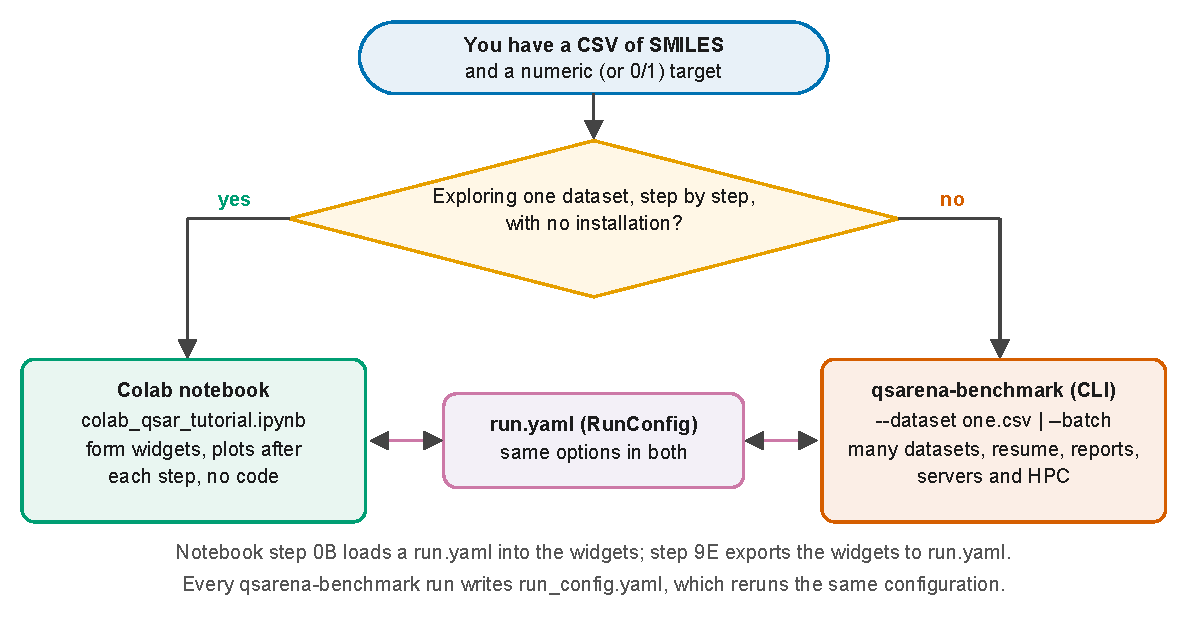
\includegraphics[width=0.95\linewidth,height=\textheight,keepaspectratio,alt={Which entry point to use.}]{figures/additional_file_2/entry_points.pdf}

\section{2. Installation}\label{installation}

\subsection{2a. Google Colab (no installation)}\label{a.-google-colab-no-installation}

Open the notebook from the badge in the repository README, or directly:
\url{https://colab.research.google.com/github/ScottCoffin/QSARena/blob/main/portable_colab_qsar_bundle/colab_qsar_tutorial.ipynb}.
Step 0 installs what it needs into the Colab session (a runtime restart may be requested once).
Nothing is installed on your own computer.

\subsection{2b. pip}\label{b.-pip}

QSARena needs Python 3.10 or newer. The core install is CPU-only and resolves on any platform with
RDKit wheels:

\begin{Shaded}
\begin{Highlighting}[]
\ExtensionTok{python} \AttributeTok{{-}m}\NormalTok{ pip install qsarena}
\end{Highlighting}
\end{Shaded}

Heavier model families are optional extras. Install only what you need: preflight lists every
missing backend with its install command, the affected models are skipped or recorded as failed with
a remedy, and the rest of the run continues.

{\def\LTcaptype{none} % do not increment counter
\begin{longtable}[]{@{}
  >{\raggedright\arraybackslash}p{(\linewidth - 4\tabcolsep) * \real{0.3333}}
  >{\raggedright\arraybackslash}p{(\linewidth - 4\tabcolsep) * \real{0.3333}}
  >{\raggedright\arraybackslash}p{(\linewidth - 4\tabcolsep) * \real{0.3333}}@{}}
\toprule\noalign{}
\begin{minipage}[b]{\linewidth}\raggedright
Extra
\end{minipage} & \begin{minipage}[b]{\linewidth}\raggedright
Adds
\end{minipage} & \begin{minipage}[b]{\linewidth}\raggedright
Install when you want
\end{minipage} \\
\midrule\noalign{}
\endhead
\bottomrule\noalign{}
\endlastfoot
\texttt{boosting} & XGBoost, LightGBM, CatBoost & gradient-boosted trees and MapLight CatBoost
(recommended) \\
\texttt{deep} & PyTorch, TensorFlow & the ChemML MLP and the tabular CNN \\
\texttt{graph} & Chemprop v2 and helpers & Chemprop graph neural networks \\
\texttt{foundation} & TabPFN, Uni-Mol tools & TabPFN and the Uni-Mol pretrained 3D models (GPU
recommended) \\
\texttt{benchmarks} & openpyxl, pyarrow, python-dotenv & the Parquet feature store and workbook
inputs \\
\texttt{notebook} & Jupyter, ipywidgets, plotting & running the notebook locally \\
\texttt{tdc} & PyTDC & the curated TDC benchmark datasets (Python 3.10-3.12 only) \\
\texttt{all} & everything above except \texttt{tdc} and \texttt{chemml} & a full CPU installation \\
\end{longtable}
}

\begin{Shaded}
\begin{Highlighting}[]
\ExtensionTok{python} \AttributeTok{{-}m}\NormalTok{ pip install }\StringTok{"qsarena[boosting]"}
\ExtensionTok{python} \AttributeTok{{-}m}\NormalTok{ pip install }\StringTok{"qsarena[all]"}
\end{Highlighting}
\end{Shaded}

MapLight + GNN additionally needs \texttt{dgl} and \texttt{dgllife}, which are not on PyPI for most
platforms; the README section ``Installation via pip'' gives the wheel index. To work on the source
instead, clone the repository and install it in editable mode:

\begin{Shaded}
\begin{Highlighting}[]
\FunctionTok{git}\NormalTok{ clone https://github.com/ScottCoffin/QSARena.git}
\BuiltInTok{cd}\NormalTok{ QSARena}
\ExtensionTok{python} \AttributeTok{{-}m}\NormalTok{ pip install }\AttributeTok{{-}e} \StringTok{".[boosting]"}
\end{Highlighting}
\end{Shaded}

\subsection{2c. Exact reproduction of the published
environment}\label{c.-exact-reproduction-of-the-published-environment}

The repository pins the environment used for the paper: \texttt{requirements-\allowbreak{}cpu.\allowbreak{}txt} /
\texttt{requirements-\allowbreak{}cuda.\allowbreak{}txt} for pip and \texttt{environment-\allowbreak{}cpu.\allowbreak{}yml} /
\texttt{environment-\allowbreak{}cuda.\allowbreak{}yml} for conda. Use them when you need the same package versions as the
deposited benchmark, not for everyday use.

\begin{Shaded}
\begin{Highlighting}[]
\ExtensionTok{conda}\NormalTok{ env create }\AttributeTok{{-}f}\NormalTok{ environment{-}cpu.yml}
\ExtensionTok{python} \AttributeTok{{-}m}\NormalTok{ pip install }\AttributeTok{{-}r}\NormalTok{ requirements{-}cpu.txt}
\end{Highlighting}
\end{Shaded}

\subsection{2d. Checking the installation}\label{d.-checking-the-installation}

\begin{Shaded}
\begin{Highlighting}[]
\ExtensionTok{qsarena{-}benchmark} \AttributeTok{{-}{-}version}
\end{Highlighting}
\end{Shaded}

\begin{Shaded}
\begin{Highlighting}[]
\NormalTok{qsarena ...}
\end{Highlighting}
\end{Shaded}

\texttt{qsarena-\allowbreak{}benchmark\ -\/-help} lists every option, grouped into the fifteen decision groups of
Section 4:

\begin{Shaded}
\begin{Highlighting}[]
\ExtensionTok{qsarena{-}benchmark} \AttributeTok{{-}{-}help}
\end{Highlighting}
\end{Shaded}

\begin{Shaded}
\begin{Highlighting}[]
\NormalTok{usage: qsarena{-}benchmark [{-}h] [{-}{-}version] ...}
\NormalTok{...}
\NormalTok{1. Input \& columns:}
\NormalTok{...}
\NormalTok{15. Execution:}
\NormalTok{...}
\end{Highlighting}
\end{Shaded}

\subsection{2e. GPU or CPU}\label{e.-gpu-or-cpu}

Everything runs on a CPU. A CUDA GPU speeds up the deep models and is required for Uni-Mol V2. By
default (\texttt{-\/-use-\allowbreak{}gpu\ auto}) QSARena detects a GPU and, when there is none, skips Uni-Mol
and runs Chemprop and the other deep models on the CPU; the preflight check says so before any model
is trained. \texttt{-\/-use-\allowbreak{}gpu\ false} hides a GPU on purpose (useful on a shared machine);
\texttt{-\/-use-\allowbreak{}gpu\ true} treats one as present.

\section{3. Quickstart: one dataset in five minutes}\label{quickstart-one-dataset-in-five-minutes}

\texttt{qsarena-\allowbreak{}examples} copies the tutorial datasets into a folder. Run the rest of the tutorial
from inside it.

\begin{Shaded}
\begin{Highlighting}[]
\ExtensionTok{qsarena{-}examples}\NormalTok{ qsarena\_tutorial}
\BuiltInTok{cd}\NormalTok{ qsarena\_tutorial}
\end{Highlighting}
\end{Shaded}

\begin{Shaded}
\begin{Highlighting}[]
\NormalTok{Wrote 8 file(s) to ...qsarena\_tutorial}
\NormalTok{solubility.csv}
\NormalTok{bbb.csv}
\NormalTok{broken.csv}
\NormalTok{batch\_manifest.csv}
\NormalTok{batch\_dir/permeability.csv}
\NormalTok{batch\_dir/lipophilicity.csv}
\NormalTok{typo\_run.yaml}
\NormalTok{run.yaml}
\end{Highlighting}
\end{Shaded}

\texttt{solubility.\allowbreak{}csv} has an identifier column, a SMILES column and two targets:

\begin{Shaded}
\begin{Highlighting}[]
\FunctionTok{cat}\NormalTok{ solubility.csv}
\end{Highlighting}
\end{Shaded}

\begin{Shaded}
\begin{Highlighting}[]
\NormalTok{compound\_id,smiles,logS,logD}
\NormalTok{SOL{-}001,...}
\NormalTok{...}
\NormalTok{SOL{-}046,this\_is\_not\_a\_smiles,{-}3.0000,1.0000}
\NormalTok{...}
\end{Highlighting}
\end{Shaded}

One command trains and compares the models. \texttt{-\/-benchmark-\allowbreak{}profile\ quick} keeps only the
fast scikit-learn model families so this finishes in a few minutes on a laptop; leave it out to use
the full default library.

\begin{Shaded}
\begin{Highlighting}[]
\ExtensionTok{qsarena{-}benchmark} \AttributeTok{{-}{-}dataset}\NormalTok{ solubility.csv }\AttributeTok{{-}{-}target{-}col}\NormalTok{ logS }\AttributeTok{{-}{-}id{-}col}\NormalTok{ compound\_id }\DataTypeTok{\textbackslash{}}
    \AttributeTok{{-}{-}benchmark{-}profile}\NormalTok{ quick }\AttributeTok{{-}{-}output{-}dir}\NormalTok{ runs/quickstart}
\end{Highlighting}
\end{Shaded}

\begin{Shaded}
\begin{Highlighting}[]
\NormalTok{Preflight checks:}
\NormalTok{{-} solubility: 47 rows, parse rate 97.9\% (1 unparseable, 0 missing), duplicates 2.2\%, task=regression}
\NormalTok{[preflight] warning solubility: 1 SMILES (2.1\%) cannot be parsed by RDKit and will be dropped. {-}\textgreater{} Fix them in the CSV, or pass {-}{-}no{-}drop{-}unparseable to stop instead of dropping.}
\NormalTok{[preflight] warning solubility: 46 usable rows: the test split will hold about 10 molecules, so test metrics are noisy. {-}\textgreater{} ...}
\NormalTok{...}
\NormalTok{Run mode: single (1 dataset(s))}
\NormalTok{...}
\NormalTok{[1/1] solubility | stage 1/13: loading ...}
\NormalTok{...}
\NormalTok{[1/1] solubility | stage 4/13: conventional model ElasticNetCV | ...}
\NormalTok{...}
\NormalTok{[1/1] solubility | stage 13/13: ensemble (2 method(s)) | ...}
\NormalTok{[overall 1/1] status=completed | ...}
\NormalTok{...}
\NormalTok{Dataset summary: 1 completed (see dataset\_summary.csv)}
\NormalTok{Wrote benchmark outputs to runs...quickstart}
\NormalTok{...}
\NormalTok{Reports written: report.html and report.md in runs...quickstart}
\end{Highlighting}
\end{Shaded}

What happened, in order:

\begin{enumerate}
\def\labelenumi{\arabic{enumi}.}
\tightlist
\item
  \textbf{Preflight} read the file before any training: 47 rows, one SMILES that RDKit cannot parse
  (it will be dropped and reported), 2.2\% duplicated structures, and a regression task. With 46
  usable molecules the test split is tiny, and preflight says what that means for the scores.
\item
  \textbf{Stages 1-3} standardized the structures, built the molecular features and split the data
  (80/20, stratified on target quartiles), then selected features using the training split only.
\item
  \textbf{Stages 4 onward} trained one model per stage. The progress line shows the stage, elapsed
  time and an ETA for the dataset.
\item
  The run wrote its outputs and the two reports.
\end{enumerate}

The output directory holds everything:

\begin{Shaded}
\begin{Highlighting}[]
\FunctionTok{ls}\NormalTok{ runs/quickstart}
\FunctionTok{ls}\NormalTok{ runs/quickstart/solubility}
\end{Highlighting}
\end{Shaded}

\begin{Shaded}
\begin{Highlighting}[]
\NormalTok{artifact\_manifest.csv}
\NormalTok{dataset\_summary.csv}
\NormalTok{environment\_manifest.json}
\NormalTok{events.jsonl}
\NormalTok{...}
\NormalTok{preflight.json}
\NormalTok{report.html}
\NormalTok{report.md}
\NormalTok{report\_assets/}
\NormalTok{report\_data.json}
\NormalTok{run.log}
\NormalTok{run\_config.json}
\NormalTok{run\_config.yaml}
\NormalTok{...}
\NormalTok{solubility/}
\NormalTok{summary\_metrics.csv}
\NormalTok{...}
\NormalTok{applicability\_domain.csv}
\NormalTok{...}
\NormalTok{metrics.csv}
\NormalTok{predictions.csv}
\NormalTok{run\_status.json}
\NormalTok{selected\_features.csv}
\NormalTok{...}
\end{Highlighting}
\end{Shaded}

{\def\LTcaptype{none} % do not increment counter
\begin{longtable}[]{@{}
  >{\raggedright\arraybackslash}p{(\linewidth - 2\tabcolsep) * \real{0.5000}}
  >{\raggedright\arraybackslash}p{(\linewidth - 2\tabcolsep) * \real{0.5000}}@{}}
\toprule\noalign{}
\begin{minipage}[b]{\linewidth}\raggedright
File
\end{minipage} & \begin{minipage}[b]{\linewidth}\raggedright
What it is
\end{minipage} \\
\midrule\noalign{}
\endhead
\bottomrule\noalign{}
\endlastfoot
\texttt{report.\allowbreak{}html}, \texttt{report.\allowbreak{}md} & The run report (Section 7). Open \texttt{report.\allowbreak{}html} in
a browser; it is self-contained. \\
\texttt{dataset\_\allowbreak{}summary.\allowbreak{}csv} & One row per dataset: status, best model by test and by CV, error and
remedy. \\
\texttt{solubility/metrics.\allowbreak{}csv} & One row per model: train/CV/test metrics, runtime, parameters,
split hashes. \\
\texttt{solubility/predictions.\allowbreak{}csv} & Every train and test prediction, with your
\texttt{compound\_\allowbreak{}id} in the \texttt{id} column. \\
\texttt{solubility/applicability\_\allowbreak{}domain.\allowbreak{}csv} & Per test molecule: in or out of the applicability
domain (Section 8). \\
\texttt{run\_\allowbreak{}config.\allowbreak{}yaml} & The fully resolved configuration; reruns this exact run (Section 9). \\
\texttt{run.\allowbreak{}log}, \texttt{events.\allowbreak{}jsonl} & The console transcript and a machine-readable event stream
(Section 7). \\
\end{longtable}
}

\textbf{The same in the notebook (three clicks).} Open the notebook in Colab (Section 2a), choose
\emph{Runtime \textgreater{} Run all}, and it works through its built-in example dataset step by
step. Some optional deep-learning steps install packages and may ask for one runtime restart; run
again from step 0 afterwards. For your own data, set \texttt{data\_\allowbreak{}source} to
\texttt{Upload\ CSV/XLSX\ (Colab\ only)} in step 1A.

\section{4. The decision reference}\label{the-decision-reference}

Every choice QSARena makes is one option of \texttt{RunConfig}, in one of fifteen groups. You can
set an option in three places, and the most specific wins:

\begin{enumerate}
\def\labelenumi{\arabic{enumi}.}
\tightlist
\item
  a command-line flag, such as \texttt{-\/-test-\allowbreak{}fraction\ 0.\allowbreak{}25};
\item
  a key in a \texttt{run.\allowbreak{}yaml} passed with \texttt{-\/-config}, such as
  \texttt{split:\ \{test\_fraction:\ 0.25\}};
\item
  the built-in default.
\end{enumerate}

The notebook widget that makes the same choice is listed next to each option; options without a
widget are available on the command line and in \texttt{run.\allowbreak{}yaml} only. The complete, commented
\texttt{run.\allowbreak{}yaml} with every default is at the end of this section,
\texttt{docs/options\_\allowbreak{}reference.\allowbreak{}md} repeats every option with its full description, and a mistyped
key or value is rejected with the allowed values:

\begin{Shaded}
\begin{Highlighting}[]
\FunctionTok{cat}\NormalTok{ typo\_run.yaml}
\ExtensionTok{qsarena{-}benchmark} \AttributeTok{{-}{-}config}\NormalTok{ typo\_run.yaml}
\end{Highlighting}
\end{Shaded}

\begin{Shaded}
\begin{Highlighting}[]
\NormalTok{...}
\NormalTok{split:}
\NormalTok{  strategy: scafold}
\NormalTok{models:}
\NormalTok{  profle: quick}
\NormalTok{[error] configuration: 2 problem(s) in typo\_run.yaml:}
\NormalTok{{-} split.strategy: \textquotesingle{}scafold\textquotesingle{} is not one of target\_quartile, random, scaffold, predefined. Did you mean \textquotesingle{}scaffold\textquotesingle{}?}
\NormalTok{{-} models.profle: unknown option in typo\_run.yaml. Did you mean \textquotesingle{}models.profile\textquotesingle{}? See docs/options\_reference.md for every key.}
\end{Highlighting}
\end{Shaded}

The starter \texttt{run.\allowbreak{}yaml} written by \texttt{qsarena-\allowbreak{}examples} sets a handful of options and
leaves the rest at their defaults:

\begin{Shaded}
\begin{Highlighting}[]
\FunctionTok{cat}\NormalTok{ run.yaml}
\end{Highlighting}
\end{Shaded}

\begin{Shaded}
\begin{Highlighting}[]
\NormalTok{...}
\NormalTok{run:}
\NormalTok{  output\_dir: runs/solubility\_config}
\NormalTok{input:}
\NormalTok{  path: solubility.csv}
\NormalTok{...}
\NormalTok{standardize:}
\NormalTok{  strip\_salts: true}
\NormalTok{  deduplicate: canonical\_smiles}
\NormalTok{models:}
\NormalTok{  profile: quick}
\NormalTok{...}
\end{Highlighting}
\end{Shaded}

\begin{Shaded}
\begin{Highlighting}[]
\ExtensionTok{qsarena{-}benchmark} \AttributeTok{{-}{-}config}\NormalTok{ run.yaml}
\end{Highlighting}
\end{Shaded}

\begin{Shaded}
\begin{Highlighting}[]
\NormalTok{...}
\NormalTok{Config file: ...run.yaml (11 key(s) set; CLI flags override them)}
\NormalTok{...}
\NormalTok{[info] solubility: dropped 1 unparseable SMILES.}
\NormalTok{[info] solubility: deduplicate=canonical\_smiles removed 2 row(s).}
\NormalTok{...}
\NormalTok{Dataset summary: 1 completed (see dataset\_summary.csv)}
\end{Highlighting}
\end{Shaded}

Paths inside a \texttt{run.\allowbreak{}yaml} are relative to the file itself. Any flag added to the command
overrides the file, for example
\texttt{qsarena-\allowbreak{}benchmark\ -\/-config\ run.\allowbreak{}yaml\ -\/-test-\allowbreak{}fraction\ 0.\allowbreak{}3}.

\subsection{4.1 Input \& columns}\label{input-columns}

\emph{What it controls:} which file(s) to read, which columns hold the SMILES, the target and an
identifier, and whether the task is regression or classification. \emph{Defaults:} the SMILES and
target columns are auto-detected from common names (\texttt{smiles}, \texttt{SMILES},
\texttt{canonical\_\allowbreak{}smiles}, \texttt{target}, \texttt{TARGET}, \ldots); the task is \texttt{auto} (a
target with exactly two values is classification). \emph{When to change:} name the columns whenever
auto-detection guesses wrong or your file has several candidate columns; give \texttt{-\/-id-\allowbreak{}col} to
carry compound IDs into \texttt{predictions.\allowbreak{}csv}; list several targets
(\texttt{-\/-target-\allowbreak{}col\ t1\ -\/-target-\allowbreak{}col\ t2}, or \texttt{target\_col:\ {[}t1,\ t2{]}}) to model
each separately; binarize a continuous measurement with \texttt{-\/-classification-\allowbreak{}threshold}
(values at or above the threshold become 1). \texttt{target\_\allowbreak{}transform:\ auto} log10-transforms a
user regression target only when every value is positive; use \texttt{raw} to keep the scale.
\texttt{minimum\_\allowbreak{}rows} (default 20) skips datasets too small to split.

{\def\LTcaptype{none} % do not increment counter
\begin{longtable}[]{@{}
  >{\raggedright\arraybackslash}p{(\linewidth - 8\tabcolsep) * \real{0.2400}}
  >{\raggedright\arraybackslash}p{(\linewidth - 8\tabcolsep) * \real{0.1600}}
  >{\raggedright\arraybackslash}p{(\linewidth - 8\tabcolsep) * \real{0.2400}}
  >{\raggedright\arraybackslash}p{(\linewidth - 8\tabcolsep) * \real{0.2000}}
  >{\raggedright\arraybackslash}p{(\linewidth - 8\tabcolsep) * \real{0.1600}}@{}}
\toprule\noalign{}
\begin{minipage}[b]{\linewidth}\raggedright
Key
\end{minipage} & \begin{minipage}[b]{\linewidth}\raggedright
Default
\end{minipage} & \begin{minipage}[b]{\linewidth}\raggedright
Allowed values
\end{minipage} & \begin{minipage}[b]{\linewidth}\raggedright
CLI flag
\end{minipage} & \begin{minipage}[b]{\linewidth}\raggedright
Notebook widget
\end{minipage} \\
\midrule\noalign{}
\endhead
\bottomrule\noalign{}
\endlastfoot
\texttt{input.\allowbreak{}path} & \texttt{null} & path/name or list & \texttt{-\/-dataset} & CLI / run.yaml
only \\
\texttt{input.\allowbreak{}smiles\_\allowbreak{}col} & \texttt{null} (auto-detect (QSAR\_READY\_SMILES, canonical\_smiles,
SMILES, smiles, Smiles)) & text & \texttt{-\/-smiles-\allowbreak{}col} & \texttt{smiles\_\allowbreak{}column} \\
\texttt{input.\allowbreak{}target\_\allowbreak{}col} & \texttt{null} (auto-detect (TARGET, target, Target, \ldots)) &
path/name or list & \texttt{-\/-target-\allowbreak{}col} & \texttt{target\_\allowbreak{}column} \\
\texttt{input.\allowbreak{}id\_\allowbreak{}col} & \texttt{null} & text & \texttt{-\/-id-\allowbreak{}col} & CLI / run.yaml only \\
\texttt{input.\allowbreak{}task} & \texttt{auto} & \texttt{auto}, \texttt{regression}, \texttt{classification} &
\texttt{-\/-task} & CLI / run.yaml only \\
\texttt{input.\allowbreak{}classification\_\allowbreak{}threshold} & \texttt{null} & float &
\texttt{-\/-classification-\allowbreak{}threshold} & CLI / run.yaml only \\
\texttt{input.\allowbreak{}target\_\allowbreak{}transform} & \texttt{auto} & \texttt{auto}, \texttt{raw}, \texttt{log10} &
\texttt{-\/-target-\allowbreak{}transform} & CLI / run.yaml only \\
\texttt{input.\allowbreak{}minimum\_\allowbreak{}rows} & \texttt{20} & int (\textgreater= 2) & \texttt{-\/-minimum-\allowbreak{}rows} & CLI
/ run.yaml only \\
\texttt{input.\allowbreak{}row\_\allowbreak{}limit} & \texttt{0} & int (\textgreater= 0) & \texttt{-\/-row-\allowbreak{}limit} & CLI /
run.yaml only \\
\end{longtable}
}

\subsection{4.2 Standardization}\label{standardization}

\emph{What it controls:} what happens to each structure before featurization. \emph{Default:}
unparseable SMILES are dropped and counted; nothing else is changed. \emph{When to change:} turn on
\texttt{strip\_\allowbreak{}salts} for data exported from registration systems (counter-ions otherwise become
features), \texttt{normalize\_\allowbreak{}charges} when the same compound appears in several protonation states,
and \texttt{deduplicate:\ canonical\_\allowbreak{}smiles} whenever a structure can appear more than once, so that
one molecule cannot end up in both the training and the test split (preflight warns above 5\%
duplicates). \texttt{-\/-no-\allowbreak{}drop-\allowbreak{}unparseable} stops the dataset instead of dropping rows, for
pipelines where silently losing data is unacceptable (see Section 10).

{\def\LTcaptype{none} % do not increment counter
\begin{longtable}[]{@{}
  >{\raggedright\arraybackslash}p{(\linewidth - 8\tabcolsep) * \real{0.2400}}
  >{\raggedright\arraybackslash}p{(\linewidth - 8\tabcolsep) * \real{0.1600}}
  >{\raggedright\arraybackslash}p{(\linewidth - 8\tabcolsep) * \real{0.2400}}
  >{\raggedright\arraybackslash}p{(\linewidth - 8\tabcolsep) * \real{0.2000}}
  >{\raggedright\arraybackslash}p{(\linewidth - 8\tabcolsep) * \real{0.1600}}@{}}
\toprule\noalign{}
\begin{minipage}[b]{\linewidth}\raggedright
Key
\end{minipage} & \begin{minipage}[b]{\linewidth}\raggedright
Default
\end{minipage} & \begin{minipage}[b]{\linewidth}\raggedright
Allowed values
\end{minipage} & \begin{minipage}[b]{\linewidth}\raggedright
CLI flag
\end{minipage} & \begin{minipage}[b]{\linewidth}\raggedright
Notebook widget
\end{minipage} \\
\midrule\noalign{}
\endhead
\bottomrule\noalign{}
\endlastfoot
\texttt{standardize.\allowbreak{}drop\_\allowbreak{}unparseable} & \texttt{true} & true / false &
\texttt{-\/-drop-\allowbreak{}unparseable\ /\ -\/-no-\allowbreak{}drop-\allowbreak{}unparseable} & CLI / run.yaml only \\
\texttt{standardize.\allowbreak{}strip\_\allowbreak{}salts} & \texttt{false} & true / false &
\texttt{-\/-strip-\allowbreak{}salts\ /\ -\/-no-\allowbreak{}strip-\allowbreak{}salts} & CLI / run.yaml only \\
\texttt{standardize.\allowbreak{}normalize\_\allowbreak{}charges} & \texttt{false} & true / false &
\texttt{-\/-normalize-\allowbreak{}charges\ /\ -\/-no-\allowbreak{}normalize-\allowbreak{}charges} & CLI / run.yaml only \\
\texttt{standardize.\allowbreak{}normalize\_\allowbreak{}tautomers} & \texttt{false} & true / false &
\texttt{-\/-normalize-\allowbreak{}tautomers\ /\ -\/-no-\allowbreak{}normalize-\allowbreak{}tautomers} & CLI / run.yaml only \\
\texttt{standardize.\allowbreak{}deduplicate} & \texttt{"none"} & \texttt{none}, \texttt{exact},
\texttt{canonical\_\allowbreak{}smiles} & \texttt{-\/-deduplicate} &
\texttt{collapse\_\allowbreak{}duplicate\_\allowbreak{}canonical\_\allowbreak{}smiles} \\
\end{longtable}
}

\subsection{4.3 Featurization}\label{featurization}

\emph{What it controls:} the molecular representations concatenated into the feature matrix: nine
fingerprint and descriptor families plus the MapLight-classic composite (Morgan counts, Avalon
counts, ErG and a panel of RDKit descriptors). \emph{Default:} all ten, 1024-bit fingerprints, with
feature caching on. \emph{When to change:} drop families to make runs faster or to test which
representation carries the signal; turn the caches off only to measure featurization time. Caches
are keyed by the molecules and the settings, so they are always safe to reuse.

{\def\LTcaptype{none} % do not increment counter
\begin{longtable}[]{@{}
  >{\raggedright\arraybackslash}p{(\linewidth - 8\tabcolsep) * \real{0.2400}}
  >{\raggedright\arraybackslash}p{(\linewidth - 8\tabcolsep) * \real{0.1600}}
  >{\raggedright\arraybackslash}p{(\linewidth - 8\tabcolsep) * \real{0.2400}}
  >{\raggedright\arraybackslash}p{(\linewidth - 8\tabcolsep) * \real{0.2000}}
  >{\raggedright\arraybackslash}p{(\linewidth - 8\tabcolsep) * \real{0.1600}}@{}}
\toprule\noalign{}
\begin{minipage}[b]{\linewidth}\raggedright
Key
\end{minipage} & \begin{minipage}[b]{\linewidth}\raggedright
Default
\end{minipage} & \begin{minipage}[b]{\linewidth}\raggedright
Allowed values
\end{minipage} & \begin{minipage}[b]{\linewidth}\raggedright
CLI flag
\end{minipage} & \begin{minipage}[b]{\linewidth}\raggedright
Notebook widget
\end{minipage} \\
\midrule\noalign{}
\endhead
\bottomrule\noalign{}
\endlastfoot
\texttt{features.\allowbreak{}families} &
\texttt{{[}morgan,\ ecfp6,\ fcfp6,\ layered,\ atom\_pair,\ topological\_torsion,\ rdk\_path,\ maccs,\ rdkit{]}}
& list of \texttt{morgan}, \texttt{ecfp6}, \texttt{fcfp6}, \texttt{layered}, \texttt{atom\_\allowbreak{}pair},
\texttt{topological\_\allowbreak{}torsion}, \texttt{rdk\_\allowbreak{}path}, \texttt{maccs}, \texttt{rdkit}, \texttt{maplight}
& \texttt{-\/-feature-\allowbreak{}families} & \texttt{use\_\allowbreak{}morgan\_\allowbreak{}features}, \texttt{use\_\allowbreak{}ecfp6\_\allowbreak{}features},
\texttt{use\_\allowbreak{}fcfp6\_\allowbreak{}features}, \texttt{use\_\allowbreak{}layered\_\allowbreak{}features}, \texttt{use\_\allowbreak{}atom\_\allowbreak{}pair\_\allowbreak{}features},
\texttt{use\_\allowbreak{}topological\_\allowbreak{}torsion\_\allowbreak{}features}, \texttt{use\_\allowbreak{}rdk\_\allowbreak{}path\_\allowbreak{}features},
\texttt{use\_\allowbreak{}maccs\_\allowbreak{}keys}, \texttt{use\_\allowbreak{}rdkit\_\allowbreak{}descriptors} \\
\texttt{features.\allowbreak{}maplight\_\allowbreak{}classic} & \texttt{true} & true / false &
\texttt{-\/-maplight-\allowbreak{}classic\ /\ -\/-no-\allowbreak{}maplight-\allowbreak{}classic} & \texttt{use\_\allowbreak{}maplight\_\allowbreak{}classic} \\
\texttt{features.\allowbreak{}fingerprint\_\allowbreak{}bits} & \texttt{1024} & int (\textgreater= 64) &
\texttt{-\/-fingerprint-\allowbreak{}bits} & \texttt{fingerprint\_\allowbreak{}bits} \\
\texttt{features.\allowbreak{}cache} & \texttt{true} & true / false &
\texttt{-\/-enable-\allowbreak{}shared-\allowbreak{}feature-\allowbreak{}matrix-\allowbreak{}cache\ /\ -\/-reuse-\allowbreak{}shared-\allowbreak{}feature-\allowbreak{}matrix-\allowbreak{}cache} & CLI /
run.yaml only \\
\texttt{features.\allowbreak{}persistent\_\allowbreak{}store} & \texttt{true} & true / false &
\texttt{-\/-enable-\allowbreak{}persistent-\allowbreak{}feature-\allowbreak{}store\ /\ -\/-reuse-\allowbreak{}persistent-\allowbreak{}feature-\allowbreak{}store} &
\texttt{enable\_\allowbreak{}persistent\_\allowbreak{}feature\_\allowbreak{}store}, \texttt{reuse\_\allowbreak{}persistent\_\allowbreak{}feature\_\allowbreak{}store} \\
\end{longtable}
}

\subsection{4.4 Splitting}\label{splitting}

\emph{What it controls:} how the held-out test set is chosen. \emph{Default:} a random 80/20 split
stratified on target quartiles, seed 13, 5-fold CV inside the training split. \emph{When to change:}
use \texttt{scaffold} to test extrapolation to new chemical series (harder and more realistic for
prospective use), \texttt{random} for classification or when quartile stratification is impossible,
and \texttt{predefined} with \texttt{-\/-predefined-\allowbreak{}split-\allowbreak{}col} when your file already marks
train/test rows. The curated benchmark datasets always keep their published split.

{\def\LTcaptype{none} % do not increment counter
\begin{longtable}[]{@{}
  >{\raggedright\arraybackslash}p{(\linewidth - 8\tabcolsep) * \real{0.2400}}
  >{\raggedright\arraybackslash}p{(\linewidth - 8\tabcolsep) * \real{0.1600}}
  >{\raggedright\arraybackslash}p{(\linewidth - 8\tabcolsep) * \real{0.2400}}
  >{\raggedright\arraybackslash}p{(\linewidth - 8\tabcolsep) * \real{0.2000}}
  >{\raggedright\arraybackslash}p{(\linewidth - 8\tabcolsep) * \real{0.1600}}@{}}
\toprule\noalign{}
\begin{minipage}[b]{\linewidth}\raggedright
Key
\end{minipage} & \begin{minipage}[b]{\linewidth}\raggedright
Default
\end{minipage} & \begin{minipage}[b]{\linewidth}\raggedright
Allowed values
\end{minipage} & \begin{minipage}[b]{\linewidth}\raggedright
CLI flag
\end{minipage} & \begin{minipage}[b]{\linewidth}\raggedright
Notebook widget
\end{minipage} \\
\midrule\noalign{}
\endhead
\bottomrule\noalign{}
\endlastfoot
\texttt{split.\allowbreak{}strategy} & \texttt{target\_\allowbreak{}quartile} & \texttt{target\_\allowbreak{}quartile}, \texttt{random},
\texttt{scaffold}, \texttt{predefined} & \texttt{-\/-split-\allowbreak{}strategy} &
\texttt{data\_\allowbreak{}split\_\allowbreak{}strategy} \\
\texttt{split.\allowbreak{}test\_\allowbreak{}fraction} & \texttt{0.\allowbreak{}2} & float (\textgreater= 0.05, \textless= 0.5) &
\texttt{-\/-test-\allowbreak{}fraction} & \texttt{test\_\allowbreak{}fraction} \\
\texttt{split.\allowbreak{}seed} & \texttt{13} & int & \texttt{-\/-random-\allowbreak{}seed} & \texttt{model\_\allowbreak{}random\_\allowbreak{}seed} \\
\texttt{split.\allowbreak{}cv\_\allowbreak{}folds} & \texttt{5} & int (\textgreater= 2) & \texttt{-\/-cv-\allowbreak{}folds} &
\texttt{cv\_\allowbreak{}folds} \\
\texttt{split.\allowbreak{}predefined\_\allowbreak{}split\_\allowbreak{}col} & \texttt{null} & text & \texttt{-\/-predefined-\allowbreak{}split-\allowbreak{}col} &
CLI / run.yaml only \\
\end{longtable}
}

\subsection{4.5 Feature selection}\label{feature-selection}

\emph{What it controls:} the train-only filtering and selection that turns thousands of features
into a few hundred. \emph{Default:} drop constant and near-constant columns, rare or near-universal
bits and exact duplicate columns, then keep the features with non-zero ElasticNetCV coefficients (at
most 10\% of the training rows), falling back to random-forest importance for very large datasets or
on a timeout. \emph{When to change:} \texttt{rf\_\allowbreak{}fallback} skips ElasticNetCV (fast; used by the
tests); \texttt{none} keeps every column (useful for models that do their own selection, but slower
and noisier).

{\def\LTcaptype{none} % do not increment counter
\begin{longtable}[]{@{}
  >{\raggedright\arraybackslash}p{(\linewidth - 8\tabcolsep) * \real{0.2400}}
  >{\raggedright\arraybackslash}p{(\linewidth - 8\tabcolsep) * \real{0.1600}}
  >{\raggedright\arraybackslash}p{(\linewidth - 8\tabcolsep) * \real{0.2400}}
  >{\raggedright\arraybackslash}p{(\linewidth - 8\tabcolsep) * \real{0.2000}}
  >{\raggedright\arraybackslash}p{(\linewidth - 8\tabcolsep) * \real{0.1600}}@{}}
\toprule\noalign{}
\begin{minipage}[b]{\linewidth}\raggedright
Key
\end{minipage} & \begin{minipage}[b]{\linewidth}\raggedright
Default
\end{minipage} & \begin{minipage}[b]{\linewidth}\raggedright
Allowed values
\end{minipage} & \begin{minipage}[b]{\linewidth}\raggedright
CLI flag
\end{minipage} & \begin{minipage}[b]{\linewidth}\raggedright
Notebook widget
\end{minipage} \\
\midrule\noalign{}
\endhead
\bottomrule\noalign{}
\endlastfoot
\texttt{feature\_\allowbreak{}selection.\allowbreak{}method} & \texttt{elasticnetcv} & \texttt{elasticnetcv},
\texttt{rf\_\allowbreak{}fallback}, \texttt{none} & \texttt{-\/-selector-\allowbreak{}method} &
\texttt{feature\_\allowbreak{}selector\_\allowbreak{}method} \\
\texttt{feature\_\allowbreak{}selection.\allowbreak{}variance\_\allowbreak{}threshold} & \texttt{1e-\allowbreak{}08} & float (\textgreater= 0.0) &
\texttt{-\/-variance-\allowbreak{}threshold} & CLI / run.yaml only \\
\texttt{feature\_\allowbreak{}selection.\allowbreak{}binary\_\allowbreak{}prevalence\_\allowbreak{}range} & \texttt{{[}0.005,\ 0.995{]}} & {[}low,
high{]} & \texttt{-\/-binary-\allowbreak{}prevalence-\allowbreak{}range} & CLI / run.yaml only \\
\texttt{feature\_\allowbreak{}selection.\allowbreak{}drop\_\allowbreak{}duplicate\_\allowbreak{}columns} & \texttt{true} & true / false &
\texttt{-\/-drop-\allowbreak{}duplicate-\allowbreak{}columns\ /\ -\/-no-\allowbreak{}drop-\allowbreak{}duplicate-\allowbreak{}columns} & CLI / run.yaml only \\
\texttt{feature\_\allowbreak{}selection.\allowbreak{}max\_\allowbreak{}selected\_\allowbreak{}features} & \texttt{0} & int (\textgreater= 0) &
\texttt{-\/-max-\allowbreak{}selected-\allowbreak{}features} & CLI / run.yaml only \\
\texttt{feature\_\allowbreak{}selection.\allowbreak{}auto\_\allowbreak{}rf\_\allowbreak{}by\_\allowbreak{}dataset\_\allowbreak{}size} & \texttt{null} (profile default (on for
cost\_optimized/quick, off for full)) & true / false &
\texttt{-\/-selector-\allowbreak{}auto-\allowbreak{}rf-\allowbreak{}by-\allowbreak{}dataset-\allowbreak{}size\ /\ -\/-no-\allowbreak{}selector-\allowbreak{}auto-\allowbreak{}rf-\allowbreak{}by-\allowbreak{}dataset-\allowbreak{}size} & CLI /
run.yaml only \\
\texttt{feature\_\allowbreak{}selection.\allowbreak{}elasticnet\_\allowbreak{}timeout\_\allowbreak{}seconds} & \texttt{7200.\allowbreak{}0} & float (\textgreater=
1.0) & \texttt{-\/-selector-\allowbreak{}elasticnet-\allowbreak{}timeout-\allowbreak{}seconds} & CLI / run.yaml only \\
\end{longtable}
}

\subsection{4.6 Model library}\label{model-library}

\emph{What it controls:} which models are trained. \emph{Default:} the \texttt{cost\_\allowbreak{}optimized}
profile, which leaves out variants that were expensive and rarely helped in the paper's benchmark.
\texttt{full} restores them; \texttt{quick} keeps only the scikit-learn family plus fusion and
ensembles. \emph{When to change:} use \texttt{quick} for a first look or a smoke test, \texttt{full}
for a final comparison; switch whole families off with \texttt{-\/-disable-\allowbreak{}model-\allowbreak{}families} (for
example \texttt{graph\_\allowbreak{}nn,pretrained\_\allowbreak{}3d} on a laptop) or single models with
\texttt{-\/-disable-\allowbreak{}model\ "Tabular\ CNN"}.

{\def\LTcaptype{none} % do not increment counter
\begin{longtable}[]{@{}
  >{\raggedright\arraybackslash}p{(\linewidth - 8\tabcolsep) * \real{0.2400}}
  >{\raggedright\arraybackslash}p{(\linewidth - 8\tabcolsep) * \real{0.1600}}
  >{\raggedright\arraybackslash}p{(\linewidth - 8\tabcolsep) * \real{0.2400}}
  >{\raggedright\arraybackslash}p{(\linewidth - 8\tabcolsep) * \real{0.2000}}
  >{\raggedright\arraybackslash}p{(\linewidth - 8\tabcolsep) * \real{0.1600}}@{}}
\toprule\noalign{}
\begin{minipage}[b]{\linewidth}\raggedright
Key
\end{minipage} & \begin{minipage}[b]{\linewidth}\raggedright
Default
\end{minipage} & \begin{minipage}[b]{\linewidth}\raggedright
Allowed values
\end{minipage} & \begin{minipage}[b]{\linewidth}\raggedright
CLI flag
\end{minipage} & \begin{minipage}[b]{\linewidth}\raggedright
Notebook widget
\end{minipage} \\
\midrule\noalign{}
\endhead
\bottomrule\noalign{}
\endlastfoot
\texttt{models.\allowbreak{}profile} & \texttt{cost\_\allowbreak{}optimized} & \texttt{cost\_\allowbreak{}optimized}, \texttt{full},
\texttt{quick} & \texttt{-\/-benchmark-\allowbreak{}profile} & CLI / run.yaml only \\
\texttt{models.\allowbreak{}enable\_\allowbreak{}families} & all \texttt{true} & mapping of \texttt{conventional\_\allowbreak{}ml},
\texttt{gradient\_\allowbreak{}boosting}, \texttt{deep\_\allowbreak{}tabular}, \texttt{graph\_\allowbreak{}nn}, \texttt{pretrained\_\allowbreak{}3d},
\texttt{maplight\_\allowbreak{}gnn}, \texttt{fusion}, \texttt{ensemble} to true/false &
\texttt{-\/-disable-\allowbreak{}model-\allowbreak{}families} & \texttt{run\_\allowbreak{}maplight\_\allowbreak{}gnn} \\
\texttt{models.\allowbreak{}disable\_\allowbreak{}models} & \texttt{{[}{]}} & text & \texttt{-\/-disable-\allowbreak{}model} & CLI /
run.yaml only \\
\texttt{models.\allowbreak{}only\_\allowbreak{}models} & \texttt{{[}{]}} & text & \texttt{-\/-only-\allowbreak{}model-\allowbreak{}names} & CLI /
run.yaml only \\
\end{longtable}
}

\subsection{4.7 GA tuning}\label{ga-tuning}

\emph{What it controls:} an optional genetic-algorithm hyperparameter search for elastic-net and
CatBoost, scored by cross-validation on the training split. \emph{Default:} off. \emph{When to
change:} \texttt{-\/-ga-\allowbreak{}models\ on} tunes the estimators in \texttt{-\/-ga-\allowbreak{}estimators};
\texttt{auto} tunes only estimators that won or improved in your most recent comparable run.
\texttt{-\/-ga-\allowbreak{}time-\allowbreak{}budget-\allowbreak{}minutes} and \texttt{-\/-ga-\allowbreak{}max-\allowbreak{}configs} cap the cost.

{\def\LTcaptype{none} % do not increment counter
\begin{longtable}[]{@{}
  >{\raggedright\arraybackslash}p{(\linewidth - 8\tabcolsep) * \real{0.2400}}
  >{\raggedright\arraybackslash}p{(\linewidth - 8\tabcolsep) * \real{0.1600}}
  >{\raggedright\arraybackslash}p{(\linewidth - 8\tabcolsep) * \real{0.2400}}
  >{\raggedright\arraybackslash}p{(\linewidth - 8\tabcolsep) * \real{0.2000}}
  >{\raggedright\arraybackslash}p{(\linewidth - 8\tabcolsep) * \real{0.1600}}@{}}
\toprule\noalign{}
\begin{minipage}[b]{\linewidth}\raggedright
Key
\end{minipage} & \begin{minipage}[b]{\linewidth}\raggedright
Default
\end{minipage} & \begin{minipage}[b]{\linewidth}\raggedright
Allowed values
\end{minipage} & \begin{minipage}[b]{\linewidth}\raggedright
CLI flag
\end{minipage} & \begin{minipage}[b]{\linewidth}\raggedright
Notebook widget
\end{minipage} \\
\midrule\noalign{}
\endhead
\bottomrule\noalign{}
\endlastfoot
\texttt{ga\_\allowbreak{}tuning.\allowbreak{}mode} & \texttt{"off"} & \texttt{off}, \texttt{on}, \texttt{auto} &
\texttt{-\/-ga-models\ off\textbackslash{}\textbar{}on\textbackslash{}\textbar{}auto} & CLI /
run.yaml only \\
\texttt{ga\_\allowbreak{}tuning.\allowbreak{}estimators} & \texttt{{[}elastic\_net,\ catboost{]}} & list of
\texttt{elastic\_\allowbreak{}net}, \texttt{catboost} & \texttt{-\/-ga-\allowbreak{}estimators} & \texttt{tune\_\allowbreak{}elasticnet},
\texttt{tune\_\allowbreak{}catboost} \\
\texttt{ga\_\allowbreak{}tuning.\allowbreak{}generations} & \texttt{12} & int (\textgreater= 1) & \texttt{-\/-ga-\allowbreak{}generations}
& \texttt{ga\_\allowbreak{}generations} \\
\texttt{ga\_\allowbreak{}tuning.\allowbreak{}population\_\allowbreak{}size} & \texttt{16} & int (\textgreater= 2) &
\texttt{-\/-ga-\allowbreak{}population-\allowbreak{}size} & \texttt{ga\_\allowbreak{}population\_\allowbreak{}size} \\
\texttt{ga\_\allowbreak{}tuning.\allowbreak{}time\_\allowbreak{}budget\_\allowbreak{}min} & \texttt{null} (no limit) & float (\textgreater= 0.0) &
\texttt{-\/-ga-\allowbreak{}time-\allowbreak{}budget-\allowbreak{}minutes} & CLI / run.yaml only \\
\texttt{ga\_\allowbreak{}tuning.\allowbreak{}max\_\allowbreak{}configs} & \texttt{null} (no limit) & int (\textgreater= 1) &
\texttt{-\/-ga-\allowbreak{}max-\allowbreak{}configs} & CLI / run.yaml only \\
\end{longtable}
}

\subsection{4.8 Deep / pretrained backends}\label{deep-pretrained-backends}

\emph{What it controls:} the ChemML MLP, the tabular CNN, TabPFN, Chemprop v2 graph networks and the
Uni-Mol pretrained 3D models. \emph{Default:} decided by the profile and by GPU detection (Uni-Mol
runs only with a GPU). \emph{When to change:} choose Chemprop variants and epochs explicitly for a
final model, lower batch sizes when a GPU runs out of memory, and set \texttt{-\/-use-\allowbreak{}gpu\ false} to
keep a shared GPU free. Each backend needs its extra from Section 2b; preflight lists what is
missing and how to install it.

{\def\LTcaptype{none} % do not increment counter
\begin{longtable}[]{@{}
  >{\raggedright\arraybackslash}p{(\linewidth - 8\tabcolsep) * \real{0.2400}}
  >{\raggedright\arraybackslash}p{(\linewidth - 8\tabcolsep) * \real{0.1600}}
  >{\raggedright\arraybackslash}p{(\linewidth - 8\tabcolsep) * \real{0.2400}}
  >{\raggedright\arraybackslash}p{(\linewidth - 8\tabcolsep) * \real{0.2000}}
  >{\raggedright\arraybackslash}p{(\linewidth - 8\tabcolsep) * \real{0.1600}}@{}}
\toprule\noalign{}
\begin{minipage}[b]{\linewidth}\raggedright
Key
\end{minipage} & \begin{minipage}[b]{\linewidth}\raggedright
Default
\end{minipage} & \begin{minipage}[b]{\linewidth}\raggedright
Allowed values
\end{minipage} & \begin{minipage}[b]{\linewidth}\raggedright
CLI flag
\end{minipage} & \begin{minipage}[b]{\linewidth}\raggedright
Notebook widget
\end{minipage} \\
\midrule\noalign{}
\endhead
\bottomrule\noalign{}
\endlastfoot
\texttt{deep.\allowbreak{}use\_\allowbreak{}gpu} & \texttt{auto} & auto / true / false & \texttt{-\/-use-\allowbreak{}gpu} & CLI / run.yaml
only \\
\texttt{deep.\allowbreak{}chemprop.\allowbreak{}variants} & \texttt{null} (profile default (cost\_optimized: attentivefp +
selected\_features; full: all five)) & list of \texttt{dmpnn}, \texttt{dmpnn\_\allowbreak{}rdkit2d},
\texttt{selected\_\allowbreak{}features}, \texttt{cmpnn}, \texttt{attentivefp} & \texttt{-\/-run-\allowbreak{}chemprop-\allowbreak{}*} &
CLI / run.yaml only \\
\texttt{deep.\allowbreak{}chemprop.\allowbreak{}epochs} & \texttt{null} (profile default (15; full: 40)) & int (\textgreater=
1) & \texttt{-\/-chemprop-\allowbreak{}epochs} & CLI / run.yaml only \\
\texttt{deep.\allowbreak{}chemprop.\allowbreak{}ensemble\_\allowbreak{}size} & \texttt{null} (profile default (1; full: 3)) & int
(\textgreater= 1) & \texttt{-\/-chemprop-\allowbreak{}ensemble-\allowbreak{}size} & CLI / run.yaml only \\
\texttt{deep.\allowbreak{}chemprop.\allowbreak{}batch\_\allowbreak{}size} & \texttt{32} & int (\textgreater= 1) &
\texttt{-\/-chemprop-\allowbreak{}batch-\allowbreak{}size} & CLI / run.yaml only \\
\texttt{deep.\allowbreak{}chemprop.\allowbreak{}seed} & \texttt{42} & int & \texttt{-\/-chemprop-\allowbreak{}random-\allowbreak{}seed} & CLI / run.yaml
only \\
\texttt{deep.\allowbreak{}unimol.\allowbreak{}v1} & \texttt{auto} & auto / true / false &
\texttt{-\/-run-\allowbreak{}unimol-\allowbreak{}v1\ /\ -\/-no-\allowbreak{}run-\allowbreak{}unimol-\allowbreak{}v1} & CLI / run.yaml only \\
\texttt{deep.\allowbreak{}unimol.\allowbreak{}v2} & \texttt{auto} & auto / true / false &
\texttt{-\/-run-\allowbreak{}unimol-\allowbreak{}v2\ /\ -\/-no-\allowbreak{}run-\allowbreak{}unimol-\allowbreak{}v2} & CLI / run.yaml only \\
\texttt{deep.\allowbreak{}unimol.\allowbreak{}v2\_\allowbreak{}size} & \texttt{84m} & \texttt{84m}, \texttt{164m}, \texttt{310m} &
\texttt{-\/-unimol-\allowbreak{}model-\allowbreak{}size} & CLI / run.yaml only \\
\texttt{deep.\allowbreak{}unimol.\allowbreak{}epochs} & \texttt{null} (10 on CPU, 20 when a GPU is detected) & int
(\textgreater= 1) & \texttt{-\/-unimol-\allowbreak{}epochs} & CLI / run.yaml only \\
\texttt{deep.\allowbreak{}unimol.\allowbreak{}lr} & \texttt{0.\allowbreak{}0001} & float (\textgreater= 0.0) &
\texttt{-\/-unimol-\allowbreak{}learning-\allowbreak{}rate} & CLI / run.yaml only \\
\texttt{deep.\allowbreak{}unimol.\allowbreak{}batch\_\allowbreak{}size} & \texttt{null} (32 on CPU; 32/64/128 by detected GPU memory) & int
(\textgreater= 1) & \texttt{-\/-unimol-\allowbreak{}batch-\allowbreak{}size} & CLI / run.yaml only \\
\texttt{deep.\allowbreak{}unimol.\allowbreak{}early\_\allowbreak{}stopping\_\allowbreak{}patience} & \texttt{5} & int (\textgreater= 1) &
\texttt{-\/-unimol-\allowbreak{}early-\allowbreak{}stopping} & CLI / run.yaml only \\
\texttt{deep.\allowbreak{}chemml.\allowbreak{}pytorch} & \texttt{true} & true / false &
\texttt{-\/-run-\allowbreak{}chemml-\allowbreak{}pytorch\ /\ -\/-no-\allowbreak{}run-\allowbreak{}chemml-\allowbreak{}pytorch} & \texttt{run\_\allowbreak{}chemml\_\allowbreak{}pytorch} \\
\texttt{deep.\allowbreak{}chemml.\allowbreak{}tensorflow} & \texttt{null} (profile default (off; full: on)) & true / false &
\texttt{-\/-run-\allowbreak{}chemml-\allowbreak{}tensorflow\ /\ -\/-no-\allowbreak{}run-\allowbreak{}chemml-\allowbreak{}tensorflow} &
\texttt{run\_\allowbreak{}chemml\_\allowbreak{}tensorflow} \\
\texttt{deep.\allowbreak{}chemml.\allowbreak{}epochs} & \texttt{80} & int (\textgreater= 1) &
\texttt{-\/-chemml-\allowbreak{}training-\allowbreak{}epochs} & \texttt{chemml\_\allowbreak{}training\_\allowbreak{}epochs} \\
\texttt{deep.\allowbreak{}tabpfn} & \texttt{null} (profile default (on; quick: off)) & true / false &
\texttt{-\/-run-\allowbreak{}tabpfn\ /\ -\/-no-\allowbreak{}run-\allowbreak{}tabpfn} & CLI / run.yaml only \\
\texttt{deep.\allowbreak{}cnn} & \texttt{null} (profile default (on; quick: off)) & true / false &
\texttt{-\/-run-\allowbreak{}cnn\ /\ -\/-no-\allowbreak{}run-\allowbreak{}cnn} & CLI / run.yaml only \\
\end{longtable}
}

\subsection{4.9 Fusion}\label{fusion}

\emph{What it controls:} combinatorial fusion analysis (CFA), which combines the best model of each
workflow family by score or rank. \emph{Default:} on, with rank combinations. CFA needs at least two
workflow families, so in the quick profile it is recorded as skipped. \emph{When to change:} rarely;
turn it off to save time when you do not need the fused model.

{\def\LTcaptype{none} % do not increment counter
\begin{longtable}[]{@{}
  >{\raggedright\arraybackslash}p{(\linewidth - 8\tabcolsep) * \real{0.2400}}
  >{\raggedright\arraybackslash}p{(\linewidth - 8\tabcolsep) * \real{0.1600}}
  >{\raggedright\arraybackslash}p{(\linewidth - 8\tabcolsep) * \real{0.2400}}
  >{\raggedright\arraybackslash}p{(\linewidth - 8\tabcolsep) * \real{0.2000}}
  >{\raggedright\arraybackslash}p{(\linewidth - 8\tabcolsep) * \real{0.1600}}@{}}
\toprule\noalign{}
\begin{minipage}[b]{\linewidth}\raggedright
Key
\end{minipage} & \begin{minipage}[b]{\linewidth}\raggedright
Default
\end{minipage} & \begin{minipage}[b]{\linewidth}\raggedright
Allowed values
\end{minipage} & \begin{minipage}[b]{\linewidth}\raggedright
CLI flag
\end{minipage} & \begin{minipage}[b]{\linewidth}\raggedright
Notebook widget
\end{minipage} \\
\midrule\noalign{}
\endhead
\bottomrule\noalign{}
\endlastfoot
\texttt{fusion.\allowbreak{}cfa\_\allowbreak{}score} & \texttt{true} & true / false & \texttt{-\/-run-\allowbreak{}cfa\ /\ -\/-no-\allowbreak{}run-\allowbreak{}cfa}
& CLI / run.yaml only \\
\texttt{fusion.\allowbreak{}cfa\_\allowbreak{}rank} & \texttt{true} & true / false &
\texttt{-\/-cfa-\allowbreak{}include-\allowbreak{}rank-\allowbreak{}combinations\ /\ -\/-no-\allowbreak{}cfa-\allowbreak{}include-\allowbreak{}rank-\allowbreak{}combinations} & CLI / run.yaml
only \\
\texttt{fusion.\allowbreak{}optimize\_\allowbreak{}metric} & \texttt{mae} & \texttt{mae}, \texttt{rmse}, \texttt{roc\_\allowbreak{}auc},
\texttt{auprc}, \texttt{balanced\_\allowbreak{}accuracy}, \texttt{mcc}, \texttt{accuracy} &
\texttt{-\/-cfa-\allowbreak{}optimize-\allowbreak{}metric} & CLI / run.yaml only \\
\end{longtable}
}

\subsection{4.10 Ensembles}\label{ensembles}

\emph{What it controls:} the ensembles built from the trained models: out-of-fold stacking with
RidgeCV and an average weighted by inverse training RMSE (a simple average is optional).
\emph{Default:} both, with members admitted using training-split predictions only
(\texttt{member\_\allowbreak{}selection\_\allowbreak{}metric:\ cv}), which keeps the test set out of every decision.
\texttt{test} reproduces the originally deposited benchmark run and is optimistically biased; use it
only for exact reproduction.

{\def\LTcaptype{none} % do not increment counter
\begin{longtable}[]{@{}
  >{\raggedright\arraybackslash}p{(\linewidth - 8\tabcolsep) * \real{0.2400}}
  >{\raggedright\arraybackslash}p{(\linewidth - 8\tabcolsep) * \real{0.1600}}
  >{\raggedright\arraybackslash}p{(\linewidth - 8\tabcolsep) * \real{0.2400}}
  >{\raggedright\arraybackslash}p{(\linewidth - 8\tabcolsep) * \real{0.2000}}
  >{\raggedright\arraybackslash}p{(\linewidth - 8\tabcolsep) * \real{0.1600}}@{}}
\toprule\noalign{}
\begin{minipage}[b]{\linewidth}\raggedright
Key
\end{minipage} & \begin{minipage}[b]{\linewidth}\raggedright
Default
\end{minipage} & \begin{minipage}[b]{\linewidth}\raggedright
Allowed values
\end{minipage} & \begin{minipage}[b]{\linewidth}\raggedright
CLI flag
\end{minipage} & \begin{minipage}[b]{\linewidth}\raggedright
Notebook widget
\end{minipage} \\
\midrule\noalign{}
\endhead
\bottomrule\noalign{}
\endlastfoot
\texttt{ensemble.\allowbreak{}oof\_\allowbreak{}stacking} & \texttt{true} & true / false & \texttt{-\/-ensemble-\allowbreak{}methods} & CLI
/ run.yaml only \\
\texttt{ensemble.\allowbreak{}inverse\_\allowbreak{}rmse\_\allowbreak{}average} & \texttt{true} & true / false &
\texttt{-\/-ensemble-\allowbreak{}methods} & CLI / run.yaml only \\
\texttt{ensemble.\allowbreak{}simple\_\allowbreak{}average} & \texttt{false} & true / false & \texttt{-\/-ensemble-\allowbreak{}methods} &
CLI / run.yaml only \\
\texttt{ensemble.\allowbreak{}member\_\allowbreak{}selection\_\allowbreak{}metric} & \texttt{cv} & \texttt{cv}, \texttt{test} &
\texttt{-\/-ensemble-\allowbreak{}member-\allowbreak{}selection-\allowbreak{}split} & CLI / run.yaml only \\
\texttt{ensemble.\allowbreak{}exclude\_\allowbreak{}negative\_\allowbreak{}test\_\allowbreak{}r2\_\allowbreak{}members} & \texttt{true} & true / false &
\texttt{-\/-ensemble-\allowbreak{}exclude-\allowbreak{}negative-\allowbreak{}test-\allowbreak{}r2-\allowbreak{}members\ /\ -\/-no-\allowbreak{}ensemble-\allowbreak{}exclude-\allowbreak{}negative-\allowbreak{}test-\allowbreak{}r2-\allowbreak{}members}
& CLI / run.yaml only \\
\texttt{ensemble.\allowbreak{}drop\_\allowbreak{}correlated\_\allowbreak{}members} & \texttt{true} & true / false &
\texttt{-\/-ensemble-\allowbreak{}drop-\allowbreak{}highly-\allowbreak{}correlated-\allowbreak{}members\ /\ -\/-no-\allowbreak{}ensemble-\allowbreak{}drop-\allowbreak{}highly-\allowbreak{}correlated-\allowbreak{}members}
& CLI / run.yaml only \\
\texttt{ensemble.\allowbreak{}max\_\allowbreak{}member\_\allowbreak{}correlation} & \texttt{0.\allowbreak{}995} & float (\textgreater= 0.0, \textless=
1.0) & \texttt{-\/-ensemble-\allowbreak{}max-\allowbreak{}train-\allowbreak{}correlation} & CLI / run.yaml only \\
\texttt{ensemble.\allowbreak{}stacking\_\allowbreak{}cv\_\allowbreak{}folds} & \texttt{5} & int (\textgreater= 2) &
\texttt{-\/-ensemble-\allowbreak{}stacking-\allowbreak{}cv-\allowbreak{}folds} & CLI / run.yaml only \\
\end{longtable}
}

\subsection{4.11 Applicability domain}\label{applicability-domain}

\emph{What it controls:} a per-test-molecule flag saying whether the model is interpolating or
extrapolating (Section 8). \emph{Default:} \texttt{both} (descriptor standardization and a
confidence measure). It never changes a metric. \emph{When to change:} \texttt{off} saves a few
seconds on very large test sets.

{\def\LTcaptype{none} % do not increment counter
\begin{longtable}[]{@{}
  >{\raggedright\arraybackslash}p{(\linewidth - 8\tabcolsep) * \real{0.2400}}
  >{\raggedright\arraybackslash}p{(\linewidth - 8\tabcolsep) * \real{0.1600}}
  >{\raggedright\arraybackslash}p{(\linewidth - 8\tabcolsep) * \real{0.2400}}
  >{\raggedright\arraybackslash}p{(\linewidth - 8\tabcolsep) * \real{0.2000}}
  >{\raggedright\arraybackslash}p{(\linewidth - 8\tabcolsep) * \real{0.1600}}@{}}
\toprule\noalign{}
\begin{minipage}[b]{\linewidth}\raggedright
Key
\end{minipage} & \begin{minipage}[b]{\linewidth}\raggedright
Default
\end{minipage} & \begin{minipage}[b]{\linewidth}\raggedright
Allowed values
\end{minipage} & \begin{minipage}[b]{\linewidth}\raggedright
CLI flag
\end{minipage} & \begin{minipage}[b]{\linewidth}\raggedright
Notebook widget
\end{minipage} \\
\midrule\noalign{}
\endhead
\bottomrule\noalign{}
\endlastfoot
\texttt{applicability\_\allowbreak{}domain.\allowbreak{}method} & \texttt{both} & \texttt{standardization},
\texttt{confidence}, \texttt{both}, \texttt{off} & \texttt{-\/-ad-\allowbreak{}method} & CLI / run.yaml only \\
\texttt{applicability\_\allowbreak{}domain.\allowbreak{}confidence\_\allowbreak{}threshold} & \texttt{0.\allowbreak{}5} & float (\textgreater= 0.0,
\textless= 1.0) & \texttt{-\/-ad-\allowbreak{}confidence-\allowbreak{}threshold} & CLI / run.yaml only \\
\texttt{applicability\_\allowbreak{}domain.\allowbreak{}knn\_\allowbreak{}quantile} & \texttt{0.\allowbreak{}95} & float (\textgreater= 0.5, \textless=
0.999) & \texttt{-\/-ad-\allowbreak{}knn-\allowbreak{}quantile} & CLI / run.yaml only \\
\end{longtable}
}

\subsection{4.12 Evaluation}\label{evaluation}

\emph{What it controls:} the primary metric used to rank models and the metrics shown in the report.
\emph{Default:} the benchmark's leaderboard metric for curated datasets, otherwise RMSE (regression)
or AUROC (classification); every metric is always written to \texttt{metrics.\allowbreak{}csv}. \emph{When to
change:} use \texttt{-\/-primary-\allowbreak{}metric\ auprc} or \texttt{balanced\_\allowbreak{}accuracy} for imbalanced
classes (preflight suggests this), or \texttt{mae} when large errors should not dominate.

{\def\LTcaptype{none} % do not increment counter
\begin{longtable}[]{@{}
  >{\raggedright\arraybackslash}p{(\linewidth - 8\tabcolsep) * \real{0.2400}}
  >{\raggedright\arraybackslash}p{(\linewidth - 8\tabcolsep) * \real{0.1600}}
  >{\raggedright\arraybackslash}p{(\linewidth - 8\tabcolsep) * \real{0.2400}}
  >{\raggedright\arraybackslash}p{(\linewidth - 8\tabcolsep) * \real{0.2000}}
  >{\raggedright\arraybackslash}p{(\linewidth - 8\tabcolsep) * \real{0.1600}}@{}}
\toprule\noalign{}
\begin{minipage}[b]{\linewidth}\raggedright
Key
\end{minipage} & \begin{minipage}[b]{\linewidth}\raggedright
Default
\end{minipage} & \begin{minipage}[b]{\linewidth}\raggedright
Allowed values
\end{minipage} & \begin{minipage}[b]{\linewidth}\raggedright
CLI flag
\end{minipage} & \begin{minipage}[b]{\linewidth}\raggedright
Notebook widget
\end{minipage} \\
\midrule\noalign{}
\endhead
\bottomrule\noalign{}
\endlastfoot
\texttt{evaluation.\allowbreak{}regression\_\allowbreak{}metrics} & \texttt{{[}rmse,\ mae,\ r2,\ spearman{]}} & list of
\texttt{rmse}, \texttt{mae}, \texttt{r2}, \texttt{spearman} & \texttt{-\/-report-\allowbreak{}regression-\allowbreak{}metrics}
& CLI / run.yaml only \\
\texttt{evaluation.\allowbreak{}classification\_\allowbreak{}metrics} &
\texttt{{[}roc\_auc,\ auprc,\ balanced\_accuracy,\ mcc{]}} & list of \texttt{roc\_\allowbreak{}auc},
\texttt{auprc}, \texttt{balanced\_\allowbreak{}accuracy}, \texttt{mcc} &
\texttt{-\/-report-\allowbreak{}classification-\allowbreak{}metrics} & CLI / run.yaml only \\
\texttt{evaluation.\allowbreak{}primary\_\allowbreak{}metric} & \texttt{auto} & \texttt{auto}, \texttt{rmse}, \texttt{mae},
\texttt{r2}, \texttt{spearman}, \texttt{pearson}, \texttt{roc\_\allowbreak{}auc}, \texttt{auprc},
\texttt{balanced\_\allowbreak{}accuracy}, \texttt{mcc}, \texttt{accuracy} & \texttt{-\/-primary-\allowbreak{}metric} & CLI /
run.yaml only \\
\end{longtable}
}

\subsection{4.13 Model-selection protocol}\label{model-selection-protocol}

\emph{What it controls:} how the report names each dataset's best model. The \textbf{test-selected}
winner has the best held-out score, which is optimistic because the test set did the choosing. The
\textbf{CV-selected} winner has the best cross-validated training score, and its test score is an
honest estimate of future performance. \emph{Default:} \texttt{both}, side by side. When they
disagree, quote the CV-selected model.

{\def\LTcaptype{none} % do not increment counter
\begin{longtable}[]{@{}
  >{\raggedright\arraybackslash}p{(\linewidth - 8\tabcolsep) * \real{0.2400}}
  >{\raggedright\arraybackslash}p{(\linewidth - 8\tabcolsep) * \real{0.1600}}
  >{\raggedright\arraybackslash}p{(\linewidth - 8\tabcolsep) * \real{0.2400}}
  >{\raggedright\arraybackslash}p{(\linewidth - 8\tabcolsep) * \real{0.2000}}
  >{\raggedright\arraybackslash}p{(\linewidth - 8\tabcolsep) * \real{0.1600}}@{}}
\toprule\noalign{}
\begin{minipage}[b]{\linewidth}\raggedright
Key
\end{minipage} & \begin{minipage}[b]{\linewidth}\raggedright
Default
\end{minipage} & \begin{minipage}[b]{\linewidth}\raggedright
Allowed values
\end{minipage} & \begin{minipage}[b]{\linewidth}\raggedright
CLI flag
\end{minipage} & \begin{minipage}[b]{\linewidth}\raggedright
Notebook widget
\end{minipage} \\
\midrule\noalign{}
\endhead
\bottomrule\noalign{}
\endlastfoot
\texttt{selection.\allowbreak{}protocol} & \texttt{both} & \texttt{test}, \texttt{cv}, \texttt{both} &
\texttt{-\/-selection-\allowbreak{}protocol} & CLI / run.yaml only \\
\end{longtable}
}

\subsection{4.14 Outputs, reporting \& caching}\label{outputs-reporting-caching}

\emph{What it controls:} where results go, how chatty the run is, which report sections are written,
and how resume treats cached work (Section 6). Both report formats are always written.
\texttt{-\/-verbosity\ quiet} shows only warnings and the final summary (the full transcript still
goes to \texttt{run.\allowbreak{}log}); \texttt{verbose} adds stage-level events to \texttt{events.\allowbreak{}jsonl} and
echoes backend commands.

{\def\LTcaptype{none} % do not increment counter
\begin{longtable}[]{@{}
  >{\raggedright\arraybackslash}p{(\linewidth - 8\tabcolsep) * \real{0.2400}}
  >{\raggedright\arraybackslash}p{(\linewidth - 8\tabcolsep) * \real{0.1600}}
  >{\raggedright\arraybackslash}p{(\linewidth - 8\tabcolsep) * \real{0.2400}}
  >{\raggedright\arraybackslash}p{(\linewidth - 8\tabcolsep) * \real{0.2000}}
  >{\raggedright\arraybackslash}p{(\linewidth - 8\tabcolsep) * \real{0.1600}}@{}}
\toprule\noalign{}
\begin{minipage}[b]{\linewidth}\raggedright
Key
\end{minipage} & \begin{minipage}[b]{\linewidth}\raggedright
Default
\end{minipage} & \begin{minipage}[b]{\linewidth}\raggedright
Allowed values
\end{minipage} & \begin{minipage}[b]{\linewidth}\raggedright
CLI flag
\end{minipage} & \begin{minipage}[b]{\linewidth}\raggedright
Notebook widget
\end{minipage} \\
\midrule\noalign{}
\endhead
\bottomrule\noalign{}
\endlastfoot
\texttt{run.\allowbreak{}output\_\allowbreak{}dir} & \texttt{null} (benchmark\_results/qsarena\_benchmark\_) & text &
\texttt{-\/-output-\allowbreak{}dir} & CLI / run.yaml only \\
\texttt{run.\allowbreak{}resume} & \texttt{true} & true / false & \texttt{-\/-resume\ /\ -\/-no-\allowbreak{}resume} & CLI /
run.yaml only \\
\texttt{run.\allowbreak{}overwrite} & \texttt{false} & true / false & \texttt{-\/-fresh} & CLI / run.yaml only \\
\texttt{run.\allowbreak{}verbosity} & \texttt{normal} & \texttt{quiet}, \texttt{normal}, \texttt{verbose},
\texttt{debug} & \texttt{-\/-verbosity} & CLI / run.yaml only \\
\texttt{report.\allowbreak{}formats} & \texttt{{[}html,\ md{]}} & list of \texttt{html}, \texttt{md} & (fixed) &
CLI / run.yaml only \\
\texttt{report.\allowbreak{}include\_\allowbreak{}plots} & \texttt{true} & true / false &
\texttt{-\/-report-\allowbreak{}plots\ /\ -\/-no-\allowbreak{}report-\allowbreak{}plots} & CLI / run.yaml only \\
\texttt{report.\allowbreak{}what\_\allowbreak{}next} & \texttt{true} & true / false &
\texttt{-\/-report-\allowbreak{}what-\allowbreak{}next\ /\ -\/-no-\allowbreak{}report-\allowbreak{}what-\allowbreak{}next} & CLI / run.yaml only \\
\texttt{report.\allowbreak{}machine\_\allowbreak{}readable\_\allowbreak{}manifest} & \texttt{true} & true / false &
\texttt{-\/-report-\allowbreak{}manifest\ /\ -\/-no-\allowbreak{}report-\allowbreak{}manifest} & CLI / run.yaml only \\
\texttt{caching.\allowbreak{}granularity} & \texttt{{[}dataset,\ stage{]}} & list of \texttt{dataset},
\texttt{stage} & \texttt{-\/-resume-\allowbreak{}granularity} & CLI / run.yaml only \\
\texttt{caching.\allowbreak{}validate\_\allowbreak{}against\_\allowbreak{}config\_\allowbreak{}signature} & \texttt{true} & true / false &
\texttt{-\/-validate-\allowbreak{}resume-\allowbreak{}signature\ /\ -\/-no-\allowbreak{}validate-\allowbreak{}resume-\allowbreak{}signature} & CLI / run.yaml only \\
\texttt{caching.\allowbreak{}atomic\_\allowbreak{}writes} & \texttt{true} & true / false &
\texttt{-\/-atomic-\allowbreak{}writes\ /\ -\/-no-\allowbreak{}atomic-\allowbreak{}writes} & CLI / run.yaml only \\
\end{longtable}
}

\subsection{4.15 Execution}\label{execution}

\emph{What it controls:} single versus batch mode, how many CPU cores and parallel datasets to use,
dry runs, and the multi-seed re-evaluation of the official TDC benchmark datasets.
\texttt{-\/-dry-\allowbreak{}run} runs the preflight checks and prints the plan and an estimated cost without
training anything:

\begin{Shaded}
\begin{Highlighting}[]
\ExtensionTok{qsarena{-}benchmark} \AttributeTok{{-}{-}dataset}\NormalTok{ solubility.csv }\AttributeTok{{-}{-}target{-}col}\NormalTok{ logS }\AttributeTok{{-}{-}output{-}dir}\NormalTok{ runs/plan }\AttributeTok{{-}{-}dry{-}run}
\end{Highlighting}
\end{Shaded}

\begin{Shaded}
\begin{Highlighting}[]
\NormalTok{Preflight checks:}
\NormalTok{...}
\NormalTok{Planned model stages (datasets x models):}
\NormalTok{{-} solubility: ... planned, ... skipped; est. \textasciitilde{}...}
\NormalTok{planned: ElasticNetCV, SVR, Random forest, ...}
\NormalTok{...}
\NormalTok{Estimated total wall{-}clock: \textasciitilde{}... (order of magnitude; method in preflight.json)}
\NormalTok{Dry run complete: no model was fitted. Plan written to runs...plan...dry\_run\_plan.md}
\end{Highlighting}
\end{Shaded}

The estimate scales the median fitting time of each model family measured in the paper's A100
benchmark run with the size of your dataset (and assumes GPU families are slower without a GPU).
Treat it as an order of magnitude.

{\def\LTcaptype{none} % do not increment counter
\begin{longtable}[]{@{}
  >{\raggedright\arraybackslash}p{(\linewidth - 8\tabcolsep) * \real{0.2400}}
  >{\raggedright\arraybackslash}p{(\linewidth - 8\tabcolsep) * \real{0.1600}}
  >{\raggedright\arraybackslash}p{(\linewidth - 8\tabcolsep) * \real{0.2400}}
  >{\raggedright\arraybackslash}p{(\linewidth - 8\tabcolsep) * \real{0.2000}}
  >{\raggedright\arraybackslash}p{(\linewidth - 8\tabcolsep) * \real{0.1600}}@{}}
\toprule\noalign{}
\begin{minipage}[b]{\linewidth}\raggedright
Key
\end{minipage} & \begin{minipage}[b]{\linewidth}\raggedright
Default
\end{minipage} & \begin{minipage}[b]{\linewidth}\raggedright
Allowed values
\end{minipage} & \begin{minipage}[b]{\linewidth}\raggedright
CLI flag
\end{minipage} & \begin{minipage}[b]{\linewidth}\raggedright
Notebook widget
\end{minipage} \\
\midrule\noalign{}
\endhead
\bottomrule\noalign{}
\endlastfoot
\texttt{run.\allowbreak{}mode} & \texttt{auto} & \texttt{auto}, \texttt{single}, \texttt{batch},
\texttt{benchmark} & \texttt{-\/-run-\allowbreak{}mode} & CLI / run.yaml only \\
\texttt{run.\allowbreak{}dry\_\allowbreak{}run} & \texttt{false} & true / false & \texttt{-\/-dry-\allowbreak{}run} & CLI / run.yaml
only \\
\texttt{run.\allowbreak{}n\_\allowbreak{}jobs} & \texttt{0} & int & \texttt{-\/-n-\allowbreak{}jobs} & CLI / run.yaml only \\
\texttt{run.\allowbreak{}parallel\_\allowbreak{}datasets} & \texttt{1} & int (\textgreater= 1) &
\texttt{-\/-parallel-\allowbreak{}datasets} & CLI / run.yaml only \\
\texttt{run.\allowbreak{}dataset\_\allowbreak{}names} & \texttt{{[}{]}} & text & \texttt{-\/-dataset-\allowbreak{}name} & CLI / run.yaml
only \\
\texttt{batch.\allowbreak{}source} & \texttt{null} & path/name or list & \texttt{-\/-batch} & CLI / run.yaml
only \\
\texttt{batch.\allowbreak{}mode} & \texttt{auto} & \texttt{auto}, \texttt{manifest}, \texttt{directory},
\texttt{list} & \texttt{-\/-batch-\allowbreak{}mode} & CLI / run.yaml only \\
\texttt{batch.\allowbreak{}continue\_\allowbreak{}on\_\allowbreak{}error} & \texttt{true} & true / false &
\texttt{-\/-continue-\allowbreak{}on-\allowbreak{}error\ /\ -\/-no-\allowbreak{}continue-\allowbreak{}on-\allowbreak{}error} & CLI / run.yaml only \\
\texttt{batch.\allowbreak{}aggregate\_\allowbreak{}summary} & \texttt{true} & true / false &
\texttt{-\/-aggregate-\allowbreak{}summary\ /\ -\/-no-\allowbreak{}aggregate-\allowbreak{}summary} & CLI / run.yaml only \\
\texttt{multiseed.\allowbreak{}enabled} & \texttt{true} & true / false &
\texttt{-\/-run-\allowbreak{}tdc22-\allowbreak{}multiseed-\allowbreak{}best\ /\ -\/-no-\allowbreak{}run-\allowbreak{}tdc22-\allowbreak{}multiseed-\allowbreak{}best} & CLI / run.yaml only \\
\texttt{multiseed.\allowbreak{}seeds} & \texttt{5} & int or list of int & \texttt{-\/-tdc22-\allowbreak{}multiseed-\allowbreak{}seeds} &
CLI / run.yaml only \\
\end{longtable}
}

\subsection{4.16 The complete run.yaml}\label{the-complete-run.yaml}

This is \texttt{configs/run.\allowbreak{}example.\allowbreak{}yaml}: every option with its default and a comment. Copy it,
delete the lines you do not need, and change the rest.

\begin{Shaded}
\begin{Highlighting}[]
\CommentTok{\# ============================================================================================}
\CommentTok{\# QSARena run configuration (generated from qsarena/config.py; do not edit by hand)}
\CommentTok{\# Use:        qsarena{-}benchmark {-}{-}config run.yaml}
\CommentTok{\# Precedence: command{-}line flags \textgreater{} this file \textgreater{} built{-}in defaults}
\CommentTok{\# Every value below is the built{-}in default. Delete the lines you do not want to change.}
\CommentTok{\# Full reference: docs/options\_reference.md}
\CommentTok{\# ============================================================================================}

\CommentTok{\# {-}{-}{-}{-}{-}{-}{-}{-}{-}{-} 14. Outputs, reporting \& caching, 15. Execution {-}{-}{-}{-}{-}{-}{-}{-}{-}{-}}
\FunctionTok{run}\KeywordTok{:}
\CommentTok{  \# single = one or more CSVs given by input.path; batch = batch.source; benchmark = the}
\CommentTok{  \# curated benchmark collection; auto picks batch if batch.source is set, else single if}
\CommentTok{  \# input.path is set, else benchmark. Choices: auto, single, batch, benchmark. CLI:}
\CommentTok{  \# {-}{-}run{-}mode.}
\AttributeTok{  }\FunctionTok{mode}\KeywordTok{:}\AttributeTok{ auto}
\CommentTok{  \# Directory that receives every artifact and the report. null =}
\CommentTok{  \# benchmark\_results/qsarena\_benchmark\_\textless{}timestamp\textgreater{}. CLI: {-}{-}output{-}dir.}
\AttributeTok{  }\FunctionTok{output\_dir}\KeywordTok{:}\AttributeTok{ }\CharTok{null}
\CommentTok{  \# Reuse completed datasets and stages already in output\_dir when their config signature}
\CommentTok{  \# matches. CLI: {-}{-}resume / {-}{-}no{-}resume.}
\AttributeTok{  }\FunctionTok{resume}\KeywordTok{:}\AttributeTok{ }\CharTok{true}
\CommentTok{  \# Ignore everything in output\_dir and recompute. The old directory is renamed to}
\CommentTok{  \# \textless{}name\textgreater{}\_superseded\_\textless{}timestamp\textgreater{}, never deleted. CLI: {-}{-}fresh.}
\AttributeTok{  }\FunctionTok{overwrite}\KeywordTok{:}\AttributeTok{ }\CharTok{false}
\CommentTok{  \# Console detail and the minimum level written to events.jsonl. run.log always keeps the}
\CommentTok{  \# full console transcript. Choices: quiet, normal, verbose, debug. CLI: {-}{-}verbosity.}
\AttributeTok{  }\FunctionTok{verbosity}\KeywordTok{:}\AttributeTok{ normal}
\CommentTok{  \# Run preflight checks, print the resolved plan and a cost estimate, write}
\CommentTok{  \# dry\_run\_plan.\{json,md\}, then exit without fitting any model. CLI: {-}{-}dry{-}run.}
\AttributeTok{  }\FunctionTok{dry\_run}\KeywordTok{:}\AttributeTok{ }\CharTok{false}
\CommentTok{  \# CPU workers for parallel{-}capable estimators. 0 or negative uses every detected core.}
\CommentTok{  \# CLI: {-}{-}n{-}jobs.}
\AttributeTok{  }\FunctionTok{n\_jobs}\KeywordTok{:}\AttributeTok{ }\DecValTok{0}
\CommentTok{  \# Datasets processed concurrently (process pool). n\_jobs is divided between workers.}
\CommentTok{  \# CLI: {-}{-}parallel{-}datasets.}
\AttributeTok{  }\FunctionTok{parallel\_datasets}\KeywordTok{:}\AttributeTok{ }\DecValTok{1}
\CommentTok{  \# Benchmark mode only: restrict the curated collection to these dataset names (list them}
\CommentTok{  \# with {-}{-}dry{-}run). CLI: {-}{-}dataset{-}name.}
\AttributeTok{  }\FunctionTok{dataset\_names}\KeywordTok{:}\AttributeTok{ }\KeywordTok{[]}

\CommentTok{\# {-}{-}{-}{-}{-}{-}{-}{-}{-}{-} 1. Input \& columns {-}{-}{-}{-}{-}{-}{-}{-}{-}{-}}
\FunctionTok{input}\KeywordTok{:}
\CommentTok{  \# CSV file (or list of CSV files) for single mode. Each file becomes one dataset named}
\CommentTok{  \# after it. CLI: {-}{-}dataset.}
\AttributeTok{  }\FunctionTok{path}\KeywordTok{:}\AttributeTok{ }\CharTok{null}
\CommentTok{  \# Column holding the SMILES strings. null = auto{-}detect (QSAR\_READY\_SMILES,}
\CommentTok{  \# canonical\_smiles, SMILES, smiles, Smiles). CLI: {-}{-}smiles{-}col.}
\AttributeTok{  }\FunctionTok{smiles\_col}\KeywordTok{:}\AttributeTok{ }\CharTok{null}
\CommentTok{  \# Target column. A list runs one dataset per target (named \textless{}file\textgreater{}\_\_\textless{}target\textgreater{}). null =}
\CommentTok{  \# auto{-}detect (TARGET, target, Target, ...). CLI: {-}{-}target{-}col.}
\AttributeTok{  }\FunctionTok{target\_col}\KeywordTok{:}\AttributeTok{ }\CharTok{null}
\CommentTok{  \# Optional identifier column, copied into the per{-}dataset predictions.csv. CLI: {-}{-}id{-}}
\CommentTok{  \# col.}
\AttributeTok{  }\FunctionTok{id\_col}\KeywordTok{:}\AttributeTok{ }\CharTok{null}
\CommentTok{  \# auto treats a target with exactly two values as classification and anything else as}
\CommentTok{  \# regression. Choices: auto, regression, classification. CLI: {-}{-}task.}
\AttributeTok{  }\FunctionTok{task}\KeywordTok{:}\AttributeTok{ auto}
\CommentTok{  \# Binarize a continuous target: value \textgreater{}= threshold becomes 1, otherwise 0. Implies task:}
\CommentTok{  \# classification. CLI: {-}{-}classification{-}threshold.}
\AttributeTok{  }\FunctionTok{classification\_threshold}\KeywordTok{:}\AttributeTok{ }\CharTok{null}
\CommentTok{  \# auto keeps curated benchmark datasets on their raw scale and log10{-}transforms a user}
\CommentTok{  \# regression target when every value is positive. Classification targets are never}
\CommentTok{  \# transformed. Choices: auto, raw, log10. CLI: {-}{-}target{-}transform.}
\AttributeTok{  }\FunctionTok{target\_transform}\KeywordTok{:}\AttributeTok{ auto}
\CommentTok{  \# Skip a dataset with fewer valid rows than this after cleanup (small{-}dataset}
\CommentTok{  \# guardrail). CLI: {-}{-}minimum{-}rows.}
\AttributeTok{  }\FunctionTok{minimum\_rows}\KeywordTok{:}\AttributeTok{ }\DecValTok{20}
\CommentTok{  \# Deterministic random subsample of this many rows (0 = use every row). Meant for smoke}
\CommentTok{  \# tests. CLI: {-}{-}row{-}limit.}
\AttributeTok{  }\FunctionTok{row\_limit}\KeywordTok{:}\AttributeTok{ }\DecValTok{0}

\CommentTok{\# {-}{-}{-}{-}{-}{-}{-}{-}{-}{-} 2. Standardization {-}{-}{-}{-}{-}{-}{-}{-}{-}{-}}
\FunctionTok{standardize}\KeywordTok{:}
\CommentTok{  \# true drops rows RDKit cannot parse and reports how many. false stops the dataset with}
\CommentTok{  \# an error listing the unparseable rows, so nothing is dropped silently. CLI: {-}{-}drop{-}}
\CommentTok{  \# unparseable / {-}{-}no{-}drop{-}unparseable.}
\AttributeTok{  }\FunctionTok{drop\_unparseable}\KeywordTok{:}\AttributeTok{ }\CharTok{true}
\CommentTok{  \# Keep only the largest organic fragment (RDKit LargestFragmentChooser). CLI: {-}{-}strip{-}}
\CommentTok{  \# salts / {-}{-}no{-}strip{-}salts.}
\AttributeTok{  }\FunctionTok{strip\_salts}\KeywordTok{:}\AttributeTok{ }\CharTok{false}
\CommentTok{  \# Neutralize charges where possible (RDKit Uncharger). CLI: {-}{-}normalize{-}charges / {-}{-}no{-}}
\CommentTok{  \# normalize{-}charges.}
\AttributeTok{  }\FunctionTok{normalize\_charges}\KeywordTok{:}\AttributeTok{ }\CharTok{false}
\CommentTok{  \# Replace each molecule with RDKit\textquotesingle{}s canonical tautomer. Slower, and can change the}
\CommentTok{  \# drawn structure. CLI: {-}{-}normalize{-}tautomers / {-}{-}no{-}normalize{-}tautomers.}
\AttributeTok{  }\FunctionTok{normalize\_tautomers}\KeywordTok{:}\AttributeTok{ }\CharTok{false}
\CommentTok{  \# none keeps every row; exact drops rows repeating both the input SMILES and the target;}
\CommentTok{  \# canonical\_smiles merges rows with the same canonical structure (mean target for}
\CommentTok{  \# regression, majority label for classification). Choices: none, exact,}
\CommentTok{  \# canonical\_smiles. CLI: {-}{-}deduplicate.}
\AttributeTok{  }\FunctionTok{deduplicate}\KeywordTok{:}\AttributeTok{ }\StringTok{"none"}

\CommentTok{\# {-}{-}{-}{-}{-}{-}{-}{-}{-}{-} 3. Featurization {-}{-}{-}{-}{-}{-}{-}{-}{-}{-}}
\FunctionTok{features}\KeywordTok{:}
\CommentTok{  \# Molecular feature families concatenated into the model matrix. \textquotesingle{}maplight\textquotesingle{} (the}
\CommentTok{  \# MapLight{-}classic composite) is normally switched by features.maplight\_classic;}
\CommentTok{  \# \textquotesingle{}avalon\textquotesingle{} and \textquotesingle{}erg\textquotesingle{} exist only inside that composite and are accepted as aliases for}
\CommentTok{  \# it. Choices: morgan, ecfp6, fcfp6, layered, atom\_pair, topological\_torsion, rdk\_path,}
\CommentTok{  \# maccs, rdkit, maplight. CLI: {-}{-}feature{-}families.}
\AttributeTok{  }\FunctionTok{families}\KeywordTok{:}\AttributeTok{ }\KeywordTok{[}\AttributeTok{morgan}\KeywordTok{,}\AttributeTok{ ecfp6}\KeywordTok{,}\AttributeTok{ fcfp6}\KeywordTok{,}\AttributeTok{ layered}\KeywordTok{,}\AttributeTok{ atom\_pair}\KeywordTok{,}\AttributeTok{ topological\_torsion}\KeywordTok{,}\AttributeTok{ rdk\_path}\KeywordTok{,}\AttributeTok{ maccs}\KeywordTok{,}\AttributeTok{ rdkit}\KeywordTok{]}
\CommentTok{  \# Add the MapLight{-}classic composite (Morgan counts + Avalon counts + ErG + RDKit}
\CommentTok{  \# descriptor panel). CLI: {-}{-}maplight{-}classic / {-}{-}no{-}maplight{-}classic.}
\AttributeTok{  }\FunctionTok{maplight\_classic}\KeywordTok{:}\AttributeTok{ }\CharTok{true}
\CommentTok{  \# Bit length of the hashed fingerprint families. CLI: {-}{-}fingerprint{-}bits.}
\AttributeTok{  }\FunctionTok{fingerprint\_bits}\KeywordTok{:}\AttributeTok{ }\DecValTok{1024}
\CommentTok{  \# Cache whole feature matrices (content{-}addressed by SMILES, families and bits) and}
\CommentTok{  \# reuse them across datasets and runs. CLI: {-}{-}enable{-}shared{-}feature{-}matrix{-}cache /}
\CommentTok{  \# {-}{-}reuse{-}shared{-}feature{-}matrix{-}cache.}
\AttributeTok{  }\FunctionTok{cache}\KeywordTok{:}\AttributeTok{ }\CharTok{true}
\CommentTok{  \# Per{-}SMILES Parquet feature store so only new molecules are featurized. CLI: {-}{-}enable{-}}
\CommentTok{  \# persistent{-}feature{-}store / {-}{-}reuse{-}persistent{-}feature{-}store.}
\AttributeTok{  }\FunctionTok{persistent\_store}\KeywordTok{:}\AttributeTok{ }\CharTok{true}

\CommentTok{\# {-}{-}{-}{-}{-}{-}{-}{-}{-}{-} 4. Splitting {-}{-}{-}{-}{-}{-}{-}{-}{-}{-}}
\FunctionTok{split}\KeywordTok{:}
\CommentTok{  \# target\_quartile stratifies the random split on target quartiles (falls back to random}
\CommentTok{  \# when that is impossible); scaffold keeps Bemis{-}Murcko scaffolds together; predefined}
\CommentTok{  \# reads split.predefined\_split\_col. Curated benchmark datasets keep their published}
\CommentTok{  \# split. Choices: target\_quartile, random, scaffold, predefined. CLI: {-}{-}split{-}strategy.}
\AttributeTok{  }\FunctionTok{strategy}\KeywordTok{:}\AttributeTok{ target\_quartile}
\CommentTok{  \# Held{-}out test fraction. CLI: {-}{-}test{-}fraction.}
\AttributeTok{  }\FunctionTok{test\_fraction}\KeywordTok{:}\AttributeTok{ }\FloatTok{0.2}
\CommentTok{  \# Seed for the split, CV folds and every seeded model. CLI: {-}{-}random{-}seed.}
\AttributeTok{  }\FunctionTok{seed}\KeywordTok{:}\AttributeTok{ }\DecValTok{13}
\CommentTok{  \# Cross{-}validation folds on the training split (CV metrics, OOF stacking, CV selection).}
\CommentTok{  \# CLI: {-}{-}cv{-}folds.}
\AttributeTok{  }\FunctionTok{cv\_folds}\KeywordTok{:}\AttributeTok{ }\DecValTok{5}
\CommentTok{  \# Column whose values are train/test (or training/holdout); used when strategy is}
\CommentTok{  \# predefined. CLI: {-}{-}predefined{-}split{-}col.}
\AttributeTok{  }\FunctionTok{predefined\_split\_col}\KeywordTok{:}\AttributeTok{ }\CharTok{null}

\CommentTok{\# {-}{-}{-}{-}{-}{-}{-}{-}{-}{-} 5. Feature selection {-}{-}{-}{-}{-}{-}{-}{-}{-}{-}}
\FunctionTok{feature\_selection}\KeywordTok{:}
\CommentTok{  \# Train{-}only selection. elasticnetcv falls back to random{-}forest importance on timeout;}
\CommentTok{  \# rf\_fallback uses random{-}forest importance directly; none keeps every column. Choices:}
\CommentTok{  \# elasticnetcv, rf\_fallback, none. CLI: {-}{-}selector{-}method.}
\AttributeTok{  }\FunctionTok{method}\KeywordTok{:}\AttributeTok{ elasticnetcv}
\CommentTok{  \# Drop columns whose training variance is at or below this value. CLI: {-}{-}variance{-}}
\CommentTok{  \# threshold.}
\AttributeTok{  }\FunctionTok{variance\_threshold}\KeywordTok{:}\AttributeTok{ }\FloatTok{1e{-}08}
\CommentTok{  \# Keep a 0/1 column only if its training prevalence lies inside [low, high]. CLI:}
\CommentTok{  \# {-}{-}binary{-}prevalence{-}range.}
\AttributeTok{  }\FunctionTok{binary\_prevalence\_range}\KeywordTok{:}\AttributeTok{ }\KeywordTok{[}\FloatTok{0.005}\KeywordTok{,}\AttributeTok{ }\FloatTok{0.995}\KeywordTok{]}
\CommentTok{  \# Drop feature columns identical to an earlier column on the training rows. CLI: {-}{-}drop{-}}
\CommentTok{  \# duplicate{-}columns / {-}{-}no{-}drop{-}duplicate{-}columns.}
\AttributeTok{  }\FunctionTok{drop\_duplicate\_columns}\KeywordTok{:}\AttributeTok{ }\CharTok{true}
\CommentTok{  \# 0 caps the selection at ceil(10\% of training rows); a positive value overrides. CLI:}
\CommentTok{  \# {-}{-}max{-}selected{-}features.}
\AttributeTok{  }\FunctionTok{max\_selected\_features}\KeywordTok{:}\AttributeTok{ }\DecValTok{0}
\CommentTok{  \# Switch to random{-}forest importance up front when ElasticNetCV is predicted to exceed}
\CommentTok{  \# its time limit. null = profile default (on for cost\_optimized/quick, off for full).}
\CommentTok{  \# CLI: {-}{-}selector{-}auto{-}rf{-}by{-}dataset{-}size / {-}{-}no{-}selector{-}auto{-}rf{-}by{-}dataset{-}size.}
\AttributeTok{  }\FunctionTok{auto\_rf\_by\_dataset\_size}\KeywordTok{:}\AttributeTok{ }\CharTok{null}
\CommentTok{  \# Wall{-}clock limit for the ElasticNetCV selector before falling back to random forest.}
\CommentTok{  \# CLI: {-}{-}selector{-}elasticnet{-}timeout{-}seconds.}
\AttributeTok{  }\FunctionTok{elasticnet\_timeout\_seconds}\KeywordTok{:}\AttributeTok{ }\FloatTok{7200.0}

\CommentTok{\# {-}{-}{-}{-}{-}{-}{-}{-}{-}{-} 6. Model library {-}{-}{-}{-}{-}{-}{-}{-}{-}{-}}
\FunctionTok{models}\KeywordTok{:}
\CommentTok{  \# cost\_optimized (default) drops historically low{-}value expensive variants; full}
\CommentTok{  \# restores them; quick keeps only the scikit{-}learn families plus fusion and ensembles}
\CommentTok{  \# (minutes on a laptop). Choices: cost\_optimized, full, quick. CLI: {-}{-}benchmark{-}profile.}
\AttributeTok{  }\FunctionTok{profile}\KeywordTok{:}\AttributeTok{ cost\_optimized}
\CommentTok{  \# Master switch per model family: conventional\_ml = scikit{-}learn models:}
\CommentTok{  \# ElasticNetCV/LogisticRegression, SVR/SVC, random forest, extra trees,}
\CommentTok{  \# HistGradientBoosting, KNN+SVM voting, AdaBoost, tabular MLP (and their GA{-}tuned}
\CommentTok{  \# versions); gradient\_boosting = XGBoost, LightGBM, CatBoost and MapLight CatBoost}
\CommentTok{  \# (needs qsarena[boosting]); deep\_tabular = ChemML MLP (PyTorch/TensorFlow), tabular CNN}
\CommentTok{  \# (TensorFlow) and TabPFN (needs qsarena[deep] / qsarena[foundation]); graph\_nn =}
\CommentTok{  \# Chemprop v2 graph variants (needs qsarena[graph]); pretrained\_3d = Uni{-}Mol V1/V2}
\CommentTok{  \# pretrained 3D models (needs qsarena[foundation]; V2 needs a GPU); maplight\_gnn =}
\CommentTok{  \# MapLight + GNN (CatBoost on MapLight features plus GIN embeddings; needs dgl/dgllife);}
\CommentTok{  \# fusion = CFA combinatorial fusion; ensemble = OOF stacking / weighted / simple{-}average}
\CommentTok{  \# ensembles. CLI: {-}{-}disable{-}model{-}families.}
\AttributeTok{  }\FunctionTok{enable\_families}\KeywordTok{:}
\AttributeTok{    }\FunctionTok{conventional\_ml}\KeywordTok{:}\AttributeTok{ }\CharTok{true}
\AttributeTok{    }\FunctionTok{gradient\_boosting}\KeywordTok{:}\AttributeTok{ }\CharTok{true}
\AttributeTok{    }\FunctionTok{deep\_tabular}\KeywordTok{:}\AttributeTok{ }\CharTok{true}
\AttributeTok{    }\FunctionTok{graph\_nn}\KeywordTok{:}\AttributeTok{ }\CharTok{true}
\AttributeTok{    }\FunctionTok{pretrained\_3d}\KeywordTok{:}\AttributeTok{ }\CharTok{true}
\AttributeTok{    }\FunctionTok{maplight\_gnn}\KeywordTok{:}\AttributeTok{ }\CharTok{true}
\AttributeTok{    }\FunctionTok{fusion}\KeywordTok{:}\AttributeTok{ }\CharTok{true}
\AttributeTok{    }\FunctionTok{ensemble}\KeywordTok{:}\AttributeTok{ }\CharTok{true}
\CommentTok{  \# Model labels to skip, exactly as they appear in metrics.csv (e.g. "Tabular CNN"). CLI:}
\CommentTok{  \# {-}{-}disable{-}model.}
\AttributeTok{  }\FunctionTok{disable\_models}\KeywordTok{:}\AttributeTok{ }\KeywordTok{[]}
\CommentTok{  \# If non{-}empty, run only these model labels (plus the ensemble when \textquotesingle{}Ensemble\textquotesingle{} is}
\CommentTok{  \# listed). CLI: {-}{-}only{-}model{-}names.}
\AttributeTok{  }\FunctionTok{only\_models}\KeywordTok{:}\AttributeTok{ }\KeywordTok{[]}

\CommentTok{\# {-}{-}{-}{-}{-}{-}{-}{-}{-}{-} 7. GA tuning {-}{-}{-}{-}{-}{-}{-}{-}{-}{-}}
\FunctionTok{ga\_tuning}\KeywordTok{:}
\CommentTok{  \# off skips GA tuning; on tunes every estimator listed; auto tunes only the estimators}
\CommentTok{  \# that won or improved in the most recent comparable run. Choices: off, on, auto. CLI:}
\CommentTok{  \# {-}{-}ga{-}models off|on|auto.}
\AttributeTok{  }\FunctionTok{mode}\KeywordTok{:}\AttributeTok{ }\StringTok{"off"}
\CommentTok{  \# Estimators tuned when mode is on (classification tunes elastic{-}net logistic}
\CommentTok{  \# regression). Choices: elastic\_net, catboost. CLI: {-}{-}ga{-}estimators.}
\AttributeTok{  }\FunctionTok{estimators}\KeywordTok{:}\AttributeTok{ }\KeywordTok{[}\AttributeTok{elastic\_net}\KeywordTok{,}\AttributeTok{ catboost}\KeywordTok{]}
\CommentTok{  \# GA generations. CLI: {-}{-}ga{-}generations.}
\AttributeTok{  }\FunctionTok{generations}\KeywordTok{:}\AttributeTok{ }\DecValTok{12}
\CommentTok{  \# Individuals per generation. CLI: {-}{-}ga{-}population{-}size.}
\AttributeTok{  }\FunctionTok{population\_size}\KeywordTok{:}\AttributeTok{ }\DecValTok{16}
\CommentTok{  \# Stop starting new generations once this many minutes have elapsed for one estimator.}
\CommentTok{  \# null = no limit. CLI: {-}{-}ga{-}time{-}budget{-}minutes.}
\AttributeTok{  }\FunctionTok{time\_budget\_min}\KeywordTok{:}\AttributeTok{ }\CharTok{null}
\CommentTok{  \# Stop after this many distinct hyperparameter configurations have been cross{-}validated.}
\CommentTok{  \# null = no limit. CLI: {-}{-}ga{-}max{-}configs.}
\AttributeTok{  }\FunctionTok{max\_configs}\KeywordTok{:}\AttributeTok{ }\CharTok{null}

\CommentTok{\# {-}{-}{-}{-}{-}{-}{-}{-}{-}{-} 8. Deep / pretrained backends {-}{-}{-}{-}{-}{-}{-}{-}{-}{-}}
\FunctionTok{deep}\KeywordTok{:}
\CommentTok{  \# auto detects a CUDA GPU; false hides any GPU (CPU only); true treats a GPU as present}
\CommentTok{  \# and warns if none is detected. CLI: {-}{-}use{-}gpu.}
\AttributeTok{  }\FunctionTok{use\_gpu}\KeywordTok{:}\AttributeTok{ auto}
\AttributeTok{  }\FunctionTok{chemprop}\KeywordTok{:}
\CommentTok{    \# Chemprop v2 variants. An empty list switches Chemprop off. Choices: dmpnn,}
\CommentTok{    \# dmpnn\_rdkit2d, selected\_features, cmpnn, attentivefp. null = profile default}
\CommentTok{    \# (cost\_optimized: attentivefp + selected\_features; full: all five). CLI: {-}{-}run{-}}
\CommentTok{    \# chemprop{-}*.}
\AttributeTok{    }\FunctionTok{variants}\KeywordTok{:}\AttributeTok{ }\CharTok{null}
\CommentTok{    \# Training epochs. null = profile default (15; full: 40). CLI: {-}{-}chemprop{-}epochs.}
\AttributeTok{    }\FunctionTok{epochs}\KeywordTok{:}\AttributeTok{ }\CharTok{null}
\CommentTok{    \# Independently initialised Chemprop models averaged per variant. null = profile}
\CommentTok{    \# default (1; full: 3). CLI: {-}{-}chemprop{-}ensemble{-}size.}
\AttributeTok{    }\FunctionTok{ensemble\_size}\KeywordTok{:}\AttributeTok{ }\CharTok{null}
\CommentTok{    \# Mini{-}batch size. CLI: {-}{-}chemprop{-}batch{-}size.}
\AttributeTok{    }\FunctionTok{batch\_size}\KeywordTok{:}\AttributeTok{ }\DecValTok{32}
\CommentTok{    \# Chemprop seed. CLI: {-}{-}chemprop{-}random{-}seed.}
\AttributeTok{    }\FunctionTok{seed}\KeywordTok{:}\AttributeTok{ }\DecValTok{42}
\AttributeTok{  }\FunctionTok{unimol}\KeywordTok{:}
\CommentTok{    \# auto runs Uni{-}Mol V1 only when a GPU is detected. CLI: {-}{-}run{-}unimol{-}v1 / {-}{-}no{-}run{-}}
\CommentTok{    \# unimol{-}v1.}
\AttributeTok{    }\FunctionTok{v1}\KeywordTok{:}\AttributeTok{ auto}
\CommentTok{    \# auto runs Uni{-}Mol V2 only when a GPU is detected (V2 always needs a GPU). CLI:}
\CommentTok{    \# {-}{-}run{-}unimol{-}v2 / {-}{-}no{-}run{-}unimol{-}v2.}
\AttributeTok{    }\FunctionTok{v2}\KeywordTok{:}\AttributeTok{ auto}
\CommentTok{    \# Uni{-}Mol V2 checkpoint size. Choices: 84m, 164m, 310m. CLI: {-}{-}unimol{-}model{-}size.}
\AttributeTok{    }\FunctionTok{v2\_size}\KeywordTok{:}\AttributeTok{ 84m}
\CommentTok{    \# Fine{-}tuning epochs. null = 10 on CPU, 20 when a GPU is detected. CLI: {-}{-}unimol{-}}
\CommentTok{    \# epochs.}
\AttributeTok{    }\FunctionTok{epochs}\KeywordTok{:}\AttributeTok{ }\CharTok{null}
\CommentTok{    \# Learning rate. CLI: {-}{-}unimol{-}learning{-}rate.}
\AttributeTok{    }\FunctionTok{lr}\KeywordTok{:}\AttributeTok{ }\FloatTok{0.0001}
\CommentTok{    \# Mini{-}batch size. null = 32 on CPU; 32/64/128 by detected GPU memory. CLI: {-}{-}unimol{-}}
\CommentTok{    \# batch{-}size.}
\AttributeTok{    }\FunctionTok{batch\_size}\KeywordTok{:}\AttributeTok{ }\CharTok{null}
\CommentTok{    \# Epochs without improvement before stopping. CLI: {-}{-}unimol{-}early{-}stopping.}
\AttributeTok{    }\FunctionTok{early\_stopping\_patience}\KeywordTok{:}\AttributeTok{ }\DecValTok{5}
\AttributeTok{  }\FunctionTok{chemml}\KeywordTok{:}
\CommentTok{    \# ChemML{-}style dense MLP on the selected descriptors (PyTorch). CLI: {-}{-}run{-}chemml{-}}
\CommentTok{    \# pytorch / {-}{-}no{-}run{-}chemml{-}pytorch.}
\AttributeTok{    }\FunctionTok{pytorch}\KeywordTok{:}\AttributeTok{ }\CharTok{true}
\CommentTok{    \# The same MLP in TensorFlow. null = profile default (off; full: on). CLI: {-}{-}run{-}}
\CommentTok{    \# chemml{-}tensorflow / {-}{-}no{-}run{-}chemml{-}tensorflow.}
\AttributeTok{    }\FunctionTok{tensorflow}\KeywordTok{:}\AttributeTok{ }\CharTok{null}
\CommentTok{    \# Training epochs. CLI: {-}{-}chemml{-}training{-}epochs.}
\AttributeTok{    }\FunctionTok{epochs}\KeywordTok{:}\AttributeTok{ }\DecValTok{80}
\CommentTok{  \# TabPFN tabular foundation model (local package on GPU, else the Prior Labs API}
\CommentTok{  \# client). null = profile default (on; quick: off). CLI: {-}{-}run{-}tabpfn / {-}{-}no{-}run{-}tabpfn.}
\AttributeTok{  }\FunctionTok{tabpfn}\KeywordTok{:}\AttributeTok{ }\CharTok{null}
\CommentTok{  \# 1{-}D CNN on the selected descriptors (needs TensorFlow). null = profile default (on;}
\CommentTok{  \# quick: off). CLI: {-}{-}run{-}cnn / {-}{-}no{-}run{-}cnn.}
\AttributeTok{  }\FunctionTok{cnn}\KeywordTok{:}\AttributeTok{ }\CharTok{null}

\CommentTok{\# {-}{-}{-}{-}{-}{-}{-}{-}{-}{-} 9. Fusion {-}{-}{-}{-}{-}{-}{-}{-}{-}{-}}
\FunctionTok{fusion}\KeywordTok{:}
\CommentTok{  \# Run CFA combinatorial fusion (score combinations) over the best model of each}
\CommentTok{  \# workflow. CLI: {-}{-}run{-}cfa / {-}{-}no{-}run{-}cfa.}
\AttributeTok{  }\FunctionTok{cfa\_score}\KeywordTok{:}\AttributeTok{ }\CharTok{true}
\CommentTok{  \# Also try CFA rank combinations (AC/WCP/WCDS). Has no effect when cfa\_score is false.}
\CommentTok{  \# CLI: {-}{-}cfa{-}include{-}rank{-}combinations / {-}{-}no{-}cfa{-}include{-}rank{-}combinations.}
\AttributeTok{  }\FunctionTok{cfa\_rank}\KeywordTok{:}\AttributeTok{ }\CharTok{true}
\CommentTok{  \# Training{-}side metric used to choose the CFA candidate (classification uses the primary}
\CommentTok{  \# metric when a regression metric is given). Choices: mae, rmse, roc\_auc, auprc,}
\CommentTok{  \# balanced\_accuracy, mcc, accuracy. CLI: {-}{-}cfa{-}optimize{-}metric.}
\AttributeTok{  }\FunctionTok{optimize\_metric}\KeywordTok{:}\AttributeTok{ mae}

\CommentTok{\# {-}{-}{-}{-}{-}{-}{-}{-}{-}{-} 10. Ensembles {-}{-}{-}{-}{-}{-}{-}{-}{-}{-}}
\FunctionTok{ensemble}\KeywordTok{:}
\CommentTok{  \# RidgeCV stacker fitted on out{-}of{-}fold training predictions. CLI: {-}{-}ensemble{-}methods.}
\AttributeTok{  }\FunctionTok{oof\_stacking}\KeywordTok{:}\AttributeTok{ }\CharTok{true}
\CommentTok{  \# Average weighted by inverse training RMSE. CLI: {-}{-}ensemble{-}methods.}
\AttributeTok{  }\FunctionTok{inverse\_rmse\_average}\KeywordTok{:}\AttributeTok{ }\CharTok{true}
\CommentTok{  \# Unweighted average of the members. CLI: {-}{-}ensemble{-}methods.}
\AttributeTok{  }\FunctionTok{simple\_average}\KeywordTok{:}\AttributeTok{ }\CharTok{false}
\CommentTok{  \# Which split may decide ensemble membership. cv (alias train) uses training{-}split}
\CommentTok{  \# predictions only and is leakage{-}free; test reproduces the originally deposited}
\CommentTok{  \# benchmark run and is optimistically biased. Choices: cv, test. CLI: {-}{-}ensemble{-}member{-}}
\CommentTok{  \# selection{-}split.}
\AttributeTok{  }\FunctionTok{member\_selection\_metric}\KeywordTok{:}\AttributeTok{ cv}
\CommentTok{  \# Drop members with negative R2 on the member{-}selection split (train when}
\CommentTok{  \# member\_selection\_metric is cv, so the default is leakage{-}free). CLI: {-}{-}ensemble{-}}
\CommentTok{  \# exclude{-}negative{-}test{-}r2{-}members / {-}{-}no{-}ensemble{-}exclude{-}negative{-}test{-}r2{-}members.}
\AttributeTok{  }\FunctionTok{exclude\_negative\_test\_r2\_members}\KeywordTok{:}\AttributeTok{ }\CharTok{true}
\CommentTok{  \# Drop one member of each pair whose training predictions are nearly identical. CLI:}
\CommentTok{  \# {-}{-}ensemble{-}drop{-}highly{-}correlated{-}members / {-}{-}no{-}ensemble{-}drop{-}highly{-}correlated{-}}
\CommentTok{  \# members.}
\AttributeTok{  }\FunctionTok{drop\_correlated\_members}\KeywordTok{:}\AttributeTok{ }\CharTok{true}
\CommentTok{  \# Correlation above which two members count as redundant. CLI: {-}{-}ensemble{-}max{-}train{-}}
\CommentTok{  \# correlation.}
\AttributeTok{  }\FunctionTok{max\_member\_correlation}\KeywordTok{:}\AttributeTok{ }\FloatTok{0.995}
\CommentTok{  \# Folds for the out{-}of{-}fold stacking predictions. CLI: {-}{-}ensemble{-}stacking{-}cv{-}folds.}
\AttributeTok{  }\FunctionTok{stacking\_cv\_folds}\KeywordTok{:}\AttributeTok{ }\DecValTok{5}

\CommentTok{\# {-}{-}{-}{-}{-}{-}{-}{-}{-}{-} 11. Applicability domain {-}{-}{-}{-}{-}{-}{-}{-}{-}{-}}
\FunctionTok{applicability\_domain}\KeywordTok{:}
\CommentTok{  \# Per{-}test{-}molecule domain flags written to applicability\_domain.csv. standardization =}
\CommentTok{  \# Roy et al. (2015) descriptor{-}range rule on the selected features; confidence =}
\CommentTok{  \# predicted{-}probability confidence |2p{-}1| of the selected model for classification, and}
\CommentTok{  \# k{-}nearest{-}neighbour Tanimoto similarity to the training set for regression.}
\CommentTok{  \# Diagnostics only: no metric changes. Choices: standardization, confidence, both, off.}
\CommentTok{  \# CLI: {-}{-}ad{-}method.}
\AttributeTok{  }\FunctionTok{method}\KeywordTok{:}\AttributeTok{ both}
\CommentTok{  \# Classification: a prediction is in{-}domain when |2p{-}1| \textgreater{}= this value (0.5 means p \textless{}=}
\CommentTok{  \# 0.25 or p \textgreater{}= 0.75). CLI: {-}{-}ad{-}confidence{-}threshold.}
\AttributeTok{  }\FunctionTok{confidence\_threshold}\KeywordTok{:}\AttributeTok{ }\FloatTok{0.5}
\CommentTok{  \# Regression: in{-}domain when the mean Tanimoto distance to the 5 nearest training}
\CommentTok{  \# molecules is at most this quantile of the training set\textquotesingle{}s own leave{-}one{-}out distances.}
\CommentTok{  \# CLI: {-}{-}ad{-}knn{-}quantile.}
\AttributeTok{  }\FunctionTok{knn\_quantile}\KeywordTok{:}\AttributeTok{ }\FloatTok{0.95}

\CommentTok{\# {-}{-}{-}{-}{-}{-}{-}{-}{-}{-} 12. Evaluation {-}{-}{-}{-}{-}{-}{-}{-}{-}{-}}
\FunctionTok{evaluation}\KeywordTok{:}
\CommentTok{  \# Metrics shown in the report tables for regression datasets. metrics.csv always}
\CommentTok{  \# contains all of them. Choices: rmse, mae, r2, spearman. CLI: {-}{-}report{-}regression{-}}
\CommentTok{  \# metrics.}
\AttributeTok{  }\FunctionTok{regression\_metrics}\KeywordTok{:}\AttributeTok{ }\KeywordTok{[}\AttributeTok{rmse}\KeywordTok{,}\AttributeTok{ mae}\KeywordTok{,}\AttributeTok{ r2}\KeywordTok{,}\AttributeTok{ spearman}\KeywordTok{]}
\CommentTok{  \# Metrics shown in the report tables for classification datasets. Choices: roc\_auc,}
\CommentTok{  \# auprc, balanced\_accuracy, mcc. CLI: {-}{-}report{-}classification{-}metrics.}
\AttributeTok{  }\FunctionTok{classification\_metrics}\KeywordTok{:}\AttributeTok{ }\KeywordTok{[}\AttributeTok{roc\_auc}\KeywordTok{,}\AttributeTok{ auprc}\KeywordTok{,}\AttributeTok{ balanced\_accuracy}\KeywordTok{,}\AttributeTok{ mcc}\KeywordTok{]}
\CommentTok{  \# Metric used to rank models, drive GA tuning and pick the best model. auto = the}
\CommentTok{  \# benchmark\textquotesingle{}s leaderboard metric, else rmse (regression) or roc\_auc (classification).}
\CommentTok{  \# Choices: auto, rmse, mae, r2, spearman, pearson, roc\_auc, auprc, balanced\_accuracy,}
\CommentTok{  \# mcc, accuracy. CLI: {-}{-}primary{-}metric.}
\AttributeTok{  }\FunctionTok{primary\_metric}\KeywordTok{:}\AttributeTok{ auto}

\CommentTok{\# {-}{-}{-}{-}{-}{-}{-}{-}{-}{-} 13. Model{-}selection protocol {-}{-}{-}{-}{-}{-}{-}{-}{-}{-}}
\FunctionTok{selection}\KeywordTok{:}
\CommentTok{  \# How the report names each dataset\textquotesingle{}s best model. test = best held{-}out score}
\CommentTok{  \# (optimistic: the test set chooses); cv = best cross{-}validated training score (honest;}
\CommentTok{  \# only models with CV metrics are eligible); both = report both side by side. Choices:}
\CommentTok{  \# test, cv, both. CLI: {-}{-}selection{-}protocol.}
\AttributeTok{  }\FunctionTok{protocol}\KeywordTok{:}\AttributeTok{ both}

\CommentTok{\# {-}{-}{-}{-}{-}{-}{-}{-}{-}{-} 14. Outputs, reporting \& caching {-}{-}{-}{-}{-}{-}{-}{-}{-}{-}}
\FunctionTok{report}\KeywordTok{:}
\CommentTok{  \# Locked: every run and batch writes both report.html and report.md. Choices: html, md.}
\AttributeTok{  }\FunctionTok{formats}\KeywordTok{:}\AttributeTok{ }\KeywordTok{[}\AttributeTok{html}\KeywordTok{,}\AttributeTok{ md}\KeywordTok{]}
\CommentTok{  \# Won{-}by{-}family, cost{-}vs{-}gap and AD{-}coverage plots (SVG, no plotting library needed).}
\CommentTok{  \# CLI: {-}{-}report{-}plots / {-}{-}no{-}report{-}plots.}
\AttributeTok{  }\FunctionTok{include\_plots}\KeywordTok{:}\AttributeTok{ }\CharTok{true}
\CommentTok{  \# Actionable "what to do next" section. CLI: {-}{-}report{-}what{-}next / {-}{-}no{-}report{-}what{-}next.}
\AttributeTok{  }\FunctionTok{what\_next}\KeywordTok{:}\AttributeTok{ }\CharTok{true}
\CommentTok{  \# Write report\_data.json alongside the reports. CLI: {-}{-}report{-}manifest / {-}{-}no{-}report{-}}
\CommentTok{  \# manifest.}
\AttributeTok{  }\FunctionTok{machine\_readable\_manifest}\KeywordTok{:}\AttributeTok{ }\CharTok{true}

\CommentTok{\# {-}{-}{-}{-}{-}{-}{-}{-}{-}{-} 15. Execution {-}{-}{-}{-}{-}{-}{-}{-}{-}{-}}
\FunctionTok{batch}\KeywordTok{:}
\CommentTok{  \# A manifest CSV (one row per dataset), a directory of CSVs, a .txt file listing CSV}
\CommentTok{  \# paths, or a list of CSV paths. CLI: {-}{-}batch.}
\AttributeTok{  }\FunctionTok{source}\KeywordTok{:}\AttributeTok{ }\CharTok{null}
\CommentTok{  \# How to read batch.source. auto: directory {-}\textgreater{} directory; .txt {-}\textgreater{} list; CSV with a}
\CommentTok{  \# \textquotesingle{}path\textquotesingle{} column {-}\textgreater{} manifest; several paths {-}\textgreater{} list. Choices: auto, manifest, directory,}
\CommentTok{  \# list. CLI: {-}{-}batch{-}mode.}
\AttributeTok{  }\FunctionTok{mode}\KeywordTok{:}\AttributeTok{ auto}
\CommentTok{  \# Record a failing dataset (status failed + error + remedy) and continue with the next}
\CommentTok{  \# one. CLI: {-}{-}continue{-}on{-}error / {-}{-}no{-}continue{-}on{-}error.}
\AttributeTok{  }\FunctionTok{continue\_on\_error}\KeywordTok{:}\AttributeTok{ }\CharTok{true}
\CommentTok{  \# Write dataset\_summary.csv with one row per dataset (status, best model, metric,}
\CommentTok{  \# error). CLI: {-}{-}aggregate{-}summary / {-}{-}no{-}aggregate{-}summary.}
\AttributeTok{  }\FunctionTok{aggregate\_summary}\KeywordTok{:}\AttributeTok{ }\CharTok{true}

\CommentTok{\# {-}{-}{-}{-}{-}{-}{-}{-}{-}{-} 15. Execution {-}{-}{-}{-}{-}{-}{-}{-}{-}{-}}
\FunctionTok{multiseed}\KeywordTok{:}
\CommentTok{  \# After the run, re{-}evaluate the selected model of each official TDC ADMET Benchmark}
\CommentTok{  \# Group dataset over several seeds. Datasets outside that group are skipped. CLI: {-}{-}run{-}}
\CommentTok{  \# tdc22{-}multiseed{-}best / {-}{-}no{-}run{-}tdc22{-}multiseed{-}best.}
\AttributeTok{  }\FunctionTok{enabled}\KeywordTok{:}\AttributeTok{ }\CharTok{true}
\CommentTok{  \# Number of seeds (n means seeds 1..n) or an explicit list of seeds. CLI:}
\CommentTok{  \# {-}{-}tdc22{-}multiseed{-}seeds.}
\AttributeTok{  }\FunctionTok{seeds}\KeywordTok{:}\AttributeTok{ }\DecValTok{5}

\CommentTok{\# {-}{-}{-}{-}{-}{-}{-}{-}{-}{-} 14. Outputs, reporting \& caching {-}{-}{-}{-}{-}{-}{-}{-}{-}{-}}
\FunctionTok{caching}\KeywordTok{:}
\CommentTok{  \# dataset reuses fully completed datasets; stage also reuses the split/feature{-}selection}
\CommentTok{  \# cache and completed model stages inside an interrupted dataset. Choices: dataset,}
\CommentTok{  \# stage. CLI: {-}{-}resume{-}granularity.}
\AttributeTok{  }\FunctionTok{granularity}\KeywordTok{:}\AttributeTok{ }\KeywordTok{[}\AttributeTok{dataset}\KeywordTok{,}\AttributeTok{ stage}\KeywordTok{]}
\CommentTok{  \# Recompute any cached model stage whose recorded config signature differs from the}
\CommentTok{  \# current one. CLI: {-}{-}validate{-}resume{-}signature / {-}{-}no{-}validate{-}resume{-}signature.}
\AttributeTok{  }\FunctionTok{validate\_against\_config\_signature}\KeywordTok{:}\AttributeTok{ }\CharTok{true}
\CommentTok{  \# Write every artifact to a temporary file and rename it into place, so an interrupted}
\CommentTok{  \# run never leaves a half{-}written file. CLI: {-}{-}atomic{-}writes / {-}{-}no{-}atomic{-}writes.}
\AttributeTok{  }\FunctionTok{atomic\_writes}\KeywordTok{:}\AttributeTok{ }\CharTok{true}
\end{Highlighting}
\end{Shaded}

\section{5. Batch mode on any number of datasets}\label{batch-mode-on-any-number-of-datasets}

\texttt{-\/-batch} runs many datasets in one command. Each dataset gets its own subdirectory, a
dataset that fails is recorded with its error and a remedy while the others continue, and
\texttt{dataset\_\allowbreak{}summary.\allowbreak{}csv} plus the report compare them all. There is no limit on the number of
datasets. A batch source is one of:

\begin{itemize}
\tightlist
\item
  a \textbf{manifest CSV} with one row per dataset (below);
\item
  a \textbf{directory}: every \texttt{*.\allowbreak{}csv} in it, with columns auto-detected;
\item
  a \textbf{list}: a \texttt{.\allowbreak{}txt} file with one CSV path per line, or several \texttt{-\/-batch}
  paths.
\end{itemize}

A manifest needs a \texttt{path} column. \texttt{dataset\_\allowbreak{}name} is optional (the file name is used
otherwise), and any other column overrides a setting for that row only. Empty cells keep the
run-level value.

{\def\LTcaptype{none} % do not increment counter
\begin{longtable}[]{@{}
  >{\raggedright\arraybackslash}p{(\linewidth - 4\tabcolsep) * \real{0.3333}}
  >{\raggedright\arraybackslash}p{(\linewidth - 4\tabcolsep) * \real{0.3333}}
  >{\raggedright\arraybackslash}p{(\linewidth - 4\tabcolsep) * \real{0.3333}}@{}}
\toprule\noalign{}
\begin{minipage}[b]{\linewidth}\raggedright
Column
\end{minipage} & \begin{minipage}[b]{\linewidth}\raggedright
Sets
\end{minipage} & \begin{minipage}[b]{\linewidth}\raggedright
Example
\end{minipage} \\
\midrule\noalign{}
\endhead
\bottomrule\noalign{}
\endlastfoot
\texttt{dataset\_\allowbreak{}name} & the output folder and report name & \texttt{solubility} \\
\texttt{path} & the CSV (relative to the manifest) & \texttt{solubility.\allowbreak{}csv} \\
\texttt{smiles\_\allowbreak{}col}, \texttt{target\_\allowbreak{}col}, \texttt{id\_\allowbreak{}col} & columns (\texttt{target\_\allowbreak{}col} may
list several, separated by \texttt{;}) & \texttt{logS} \\
\texttt{task}, \texttt{classification\_\allowbreak{}threshold}, \texttt{target\_\allowbreak{}transform},
\texttt{minimum\_\allowbreak{}rows} & Section 4.1 & \texttt{classification} \\
\texttt{split}, \texttt{test\_\allowbreak{}fraction}, \texttt{seed}, \texttt{cv\_\allowbreak{}folds},
\texttt{predefined\_\allowbreak{}split\_\allowbreak{}col} & Section 4.4 & \texttt{scaffold} \\
\texttt{primary\_\allowbreak{}metric} & Section 4.12 & \texttt{auprc} \\
any dotted \texttt{RunConfig} key & that option (lists separated by \texttt{;}) &
\texttt{models.\allowbreak{}disable\_\allowbreak{}models} \\
\end{longtable}
}

The example manifest lists three datasets. The third, \texttt{broken.\allowbreak{}csv}, has no SMILES column on
purpose:

\begin{Shaded}
\begin{Highlighting}[]
\FunctionTok{cat}\NormalTok{ batch\_manifest.csv}
\end{Highlighting}
\end{Shaded}

\begin{Shaded}
\begin{Highlighting}[]
\NormalTok{dataset\_name,path,smiles\_col,target\_col,id\_col,task,split,test\_fraction}
\NormalTok{solubility,solubility.csv,smiles,logS,compound\_id,regression,random,0.25}
\NormalTok{bbb,bbb.csv,smiles,bbb\_penetrant,molecule,classification,random,}
\NormalTok{broken,broken.csv,,,,,,}
\end{Highlighting}
\end{Shaded}

\begin{Shaded}
\begin{Highlighting}[]
\ExtensionTok{qsarena{-}benchmark} \AttributeTok{{-}{-}batch}\NormalTok{ batch\_manifest.csv }\AttributeTok{{-}{-}benchmark{-}profile}\NormalTok{ quick }\AttributeTok{{-}{-}output{-}dir}\NormalTok{ runs/batch}
\end{Highlighting}
\end{Shaded}

\begin{Shaded}
\begin{Highlighting}[]
\NormalTok{Batch source: 3 dataset(s) from batch\_manifest.csv}
\NormalTok{[fail] broken (batch\_manifest.csv row 4): broken.csv: could not infer the SMILES column ...}
\NormalTok{...}
\NormalTok{{-} solubility: 47 rows, parse rate 97.9\% (1 unparseable, 0 missing), duplicates 2.2\%, task=regression}
\NormalTok{...}
\NormalTok{{-} bbb: 44 rows, parse rate 100.0\% (0 unparseable, 0 missing), duplicates 0.0\%, task=classification, classes=\{\textquotesingle{}0\textquotesingle{}: 16, \textquotesingle{}1\textquotesingle{}: 28\}}
\NormalTok{...}
\NormalTok{Run mode: batch (2 dataset(s), 1 failed to load)}
\NormalTok{...}
\NormalTok{[overall 2/2] status=completed | ...}
\NormalTok{...}
\NormalTok{Dataset summary: 2 completed, 1 failed (see dataset\_summary.csv)}
\end{Highlighting}
\end{Shaded}

The run finishes with exit status 0 even though one dataset failed; check
\texttt{dataset\_\allowbreak{}summary.\allowbreak{}csv} (or the report) to see which datasets need attention:

\begin{Shaded}
\begin{Highlighting}[]
\FunctionTok{cat}\NormalTok{ runs/batch/dataset\_summary.csv}
\end{Highlighting}
\end{Shaded}

\begin{Shaded}
\begin{Highlighting}[]
\NormalTok{dataset,status,task,n\_rows,primary\_metric,best\_by\_test,best\_by\_test\_test\_value,best\_by\_cv,best\_by\_cv\_test\_value,best\_by\_cv\_cv\_value,n\_models\_ok,n\_models\_failed,ad\_in\_domain\_fraction,elapsed\_seconds,error,remedy,source}
\NormalTok{solubility,completed,regression,46,rmse,...}
\NormalTok{bbb,completed,classification,44,roc\_auc,...}
\NormalTok{broken,failed,...could not infer the SMILES column...,Name the column with {-}{-}smiles{-}col COLUMN.,...}
\end{Highlighting}
\end{Shaded}

The manifest's overrides were applied per dataset: \texttt{solubility} used a 25\% test split (12 of
46 molecules), \texttt{bbb} the run-level 20\% (9 of 44), and both kept their identifiers in
\texttt{predictions.\allowbreak{}csv}.

A directory works the same way without a manifest; its files must have auto-detectable column names
(here \texttt{smiles} and \texttt{target}):

\begin{Shaded}
\begin{Highlighting}[]
\ExtensionTok{qsarena{-}benchmark} \AttributeTok{{-}{-}batch}\NormalTok{ batch\_dir }\AttributeTok{{-}{-}benchmark{-}profile}\NormalTok{ quick }\AttributeTok{{-}{-}output{-}dir}\NormalTok{ runs/batch\_dir}
\end{Highlighting}
\end{Shaded}

\begin{Shaded}
\begin{Highlighting}[]
\NormalTok{Batch source: 2 dataset(s) from batch\_dir}
\NormalTok{...}
\NormalTok{Dataset summary: 2 completed (see dataset\_summary.csv)}
\end{Highlighting}
\end{Shaded}

For large batches, \texttt{-\/-parallel-\allowbreak{}datasets\ N} runs N datasets at once (CPU cores are shared
between them) and \texttt{-\/-no-\allowbreak{}continue-\allowbreak{}on-\allowbreak{}error} stops at the first failure instead of recording
it.

\section{6. Resume}\label{resume}

A long run can be stopped at any time (Ctrl+C, a closed laptop, a killed HPC job) and continued by
running \textbf{the same command again}. Nothing that finished is recomputed.

Three levels of work are cached in the output directory:

\begin{enumerate}
\def\labelenumi{\arabic{enumi}.}
\tightlist
\item
  \textbf{Completed datasets.} A dataset whose \texttt{run\_\allowbreak{}status.\allowbreak{}json} says \texttt{completed} is
  reused as a whole.
\item
  \textbf{The split and feature selection} (\texttt{stage23\_\allowbreak{}resume\_\allowbreak{}cache.\allowbreak{}pkl}), keyed by the data,
  the split and the feature and selection settings.
\item
  \textbf{Each completed model.} Every row of \texttt{metrics.\allowbreak{}csv} carries a
  \texttt{stage\_\allowbreak{}config\_\allowbreak{}signature}.
\end{enumerate}

Running the quickstart command again reuses everything:

\begin{Shaded}
\begin{Highlighting}[]
\ExtensionTok{qsarena{-}benchmark} \AttributeTok{{-}{-}dataset}\NormalTok{ solubility.csv }\AttributeTok{{-}{-}target{-}col}\NormalTok{ logS }\AttributeTok{{-}{-}id{-}col}\NormalTok{ compound\_id }\DataTypeTok{\textbackslash{}}
    \AttributeTok{{-}{-}benchmark{-}profile}\NormalTok{ quick }\AttributeTok{{-}{-}output{-}dir}\NormalTok{ runs/quickstart}
\end{Highlighting}
\end{Shaded}

\begin{Shaded}
\begin{Highlighting}[]
\NormalTok{...}
\NormalTok{Resume execution plan: 0/1 dataset(s) require model execution; 1 dataset(s) can be reused as{-}completed.}
\NormalTok{...}
\NormalTok{[1/1] solubility: already completed in ...; reusing saved outputs}
\NormalTok{[overall 1/1] status=resumed | ...}
\end{Highlighting}
\end{Shaded}

\textbf{A changed setting recomputes only what it affects.} Here only an ensemble option changes, so
the features, the split and the eight models are reused and only the two ensembles are rebuilt:

\begin{Shaded}
\begin{Highlighting}[]
\ExtensionTok{qsarena{-}benchmark} \AttributeTok{{-}{-}dataset}\NormalTok{ solubility.csv }\AttributeTok{{-}{-}target{-}col}\NormalTok{ logS }\AttributeTok{{-}{-}id{-}col}\NormalTok{ compound\_id }\DataTypeTok{\textbackslash{}}
    \AttributeTok{{-}{-}benchmark{-}profile}\NormalTok{ quick }\AttributeTok{{-}{-}output{-}dir}\NormalTok{ runs/quickstart }\AttributeTok{{-}{-}ensemble{-}max{-}train{-}correlation}\NormalTok{ 0.99}
\end{Highlighting}
\end{Shaded}

\begin{Shaded}
\begin{Highlighting}[]
\NormalTok{[resume] solubility: configuration or input changed since this dataset completed; re{-}validating each cached stage against the new config signature.}
\NormalTok{...}
\NormalTok{[resume] solubility: config signature changed for 2 cached model stage(s) (Ensemble (OOF Stacking (RidgeCV, 5{-}fold)), Ensemble (Weighted average (inverse train RMSE))); recomputing them.}
\NormalTok{...}
\NormalTok{[resume] solubility: stage 2/3 cache hit (signature match); reusing split + selected feature matrices.}
\NormalTok{...}
\NormalTok{[1/1] solubility | stage 4/13: conventional model ElasticNetCV (cached) | ...}
\NormalTok{...}
\NormalTok{[1/1] solubility | stage 13/13: ensemble (2 method(s)) | ...}
\end{Highlighting}
\end{Shaded}

Changing the data, the split, the features or the feature selection invalidates the split cache and
every model; changing a model family's own settings (for example \texttt{-\/-chemprop-\allowbreak{}epochs})
invalidates only that family, plus fusion and the ensembles, which are built from its predictions.

\textbf{Starting over.} \texttt{-\/-fresh} ignores everything in the output directory. The old
directory is renamed, not deleted, so earlier results are never lost:

\begin{Shaded}
\begin{Highlighting}[]
\ExtensionTok{qsarena{-}benchmark} \AttributeTok{{-}{-}dataset}\NormalTok{ solubility.csv }\AttributeTok{{-}{-}target{-}col}\NormalTok{ logS }\AttributeTok{{-}{-}id{-}col}\NormalTok{ compound\_id }\DataTypeTok{\textbackslash{}}
    \AttributeTok{{-}{-}benchmark{-}profile}\NormalTok{ quick }\AttributeTok{{-}{-}output{-}dir}\NormalTok{ runs/quickstart }\AttributeTok{{-}{-}fresh}
\end{Highlighting}
\end{Shaded}

\begin{Shaded}
\begin{Highlighting}[]
\NormalTok{{-}{-}fresh: moved the previous contents of runs...quickstart to runs...quickstart\_superseded\_...}
\NormalTok{...}
\NormalTok{Dataset summary: 1 completed (see dataset\_summary.csv)}
\end{Highlighting}
\end{Shaded}

\textbf{Why an interruption is safe.} Every file is written to a temporary name and then renamed
into place, so a killed run leaves either the previous complete file or the new complete file, never
half of one. On restart, the interrupted model is trained again and everything before it is reused
(the test suite kills runs mid-model and mid-batch and checks that the resumed results are
identical).

\texttt{caching.\allowbreak{}granularity} limits reuse to whole datasets (\texttt{dataset}) or also allows reuse
of stages inside an interrupted dataset (\texttt{stage}, the default);
\texttt{-\/-no-\allowbreak{}validate-\allowbreak{}resume-\allowbreak{}signature} turns the signature checks off (not recommended).

\section{7. Understanding the reports}\label{understanding-the-reports}

Every run and every batch writes \texttt{report.\allowbreak{}html} (self-contained: open it in any browser,
attach it to an email) and \texttt{report.\allowbreak{}md} (the same content as plain text, with the plots as SVG
files in \texttt{report\_\allowbreak{}assets/}). Their sections are:

\begin{itemize}
\tightlist
\item
  \textbf{Warnings}: every actionable warning of the run, each with a remedy (small datasets,
  dropped SMILES, missing backends, failed models, molecules outside the applicability domain,
  coarse leaderboard ranks).
\item
  \textbf{Datasets}: status, task, rows used, SMILES dropped, the primary metric, and the error and
  remedy of a failed dataset.
\item
  \textbf{Best model per dataset}: the test-selected and CV-selected winners side by side (Section
  4.13), with the metrics chosen in Section 4.12. CV scores are computed after feature selection on
  the same training split, so they are optimistic in absolute terms: use them to rank models, and
  quote the test score of the CV-selected model.
\item
  \textbf{Leaderboard / rank table}: for curated benchmark datasets only, the estimated rank of our
  best model against the cached published top 10. Ranks are leaderboard-equivalent only on official
  splits, and the table warns when a leaderboard has fewer than ten entries.
\item
  \textbf{Plots} (from the batch run in Section 5):
\end{itemize}

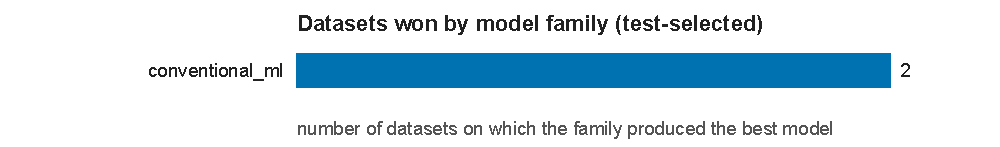
\includegraphics[width=0.95\linewidth,height=\textheight,keepaspectratio,alt={Datasets won by each model family.}]{figures/additional_file_2/won_by_family.pdf}

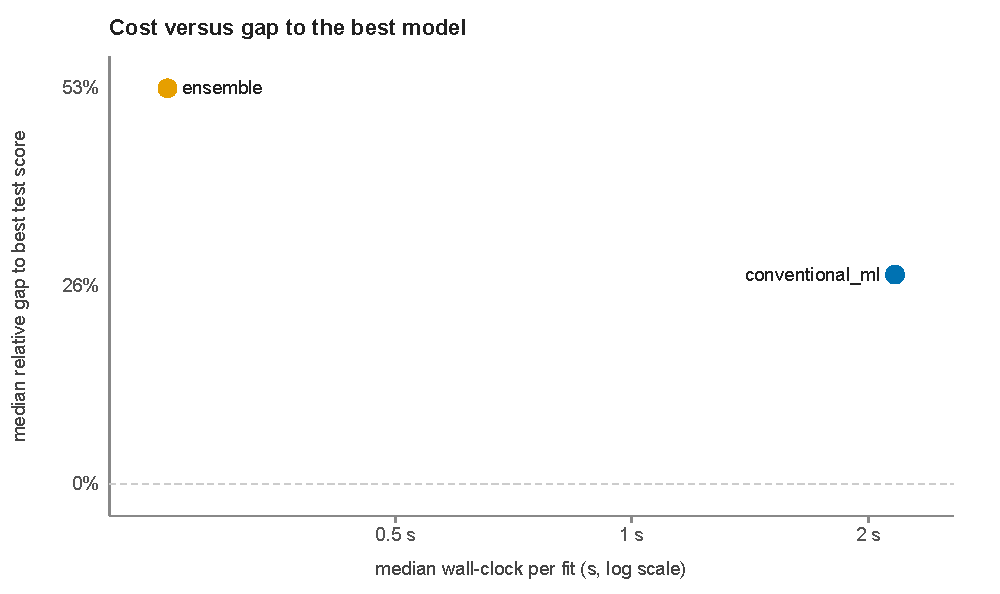
\includegraphics[width=0.95\linewidth,height=\textheight,keepaspectratio,alt={Median cost versus gap to the best model, by family.}]{figures/additional_file_2/cost_vs_gap.pdf}

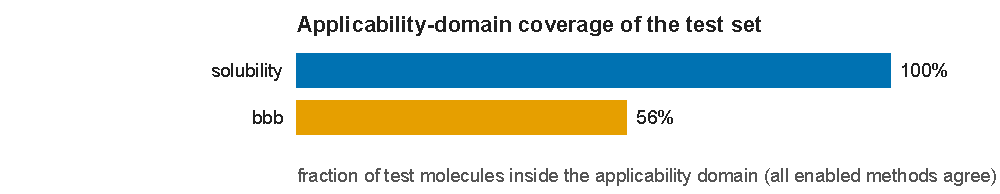
\includegraphics[width=0.95\linewidth,height=\textheight,keepaspectratio,alt={Applicability-domain coverage of each test set.}]{figures/additional_file_2/ad_coverage.pdf}

\begin{itemize}
\tightlist
\item
  \textbf{Model failures and skipped stages}: every failed model with its error and remedy, and the
  stages skipped by design (for example CFA with a single workflow family).
\item
  \textbf{What to do next}: concrete follow-ups with commands, for example repeating the run with
  other seeds, fixing a failed dataset, or running the full model library after a quick run.
\item
  \textbf{Resolved configuration}: the complete \texttt{run\_\allowbreak{}config.\allowbreak{}yaml}.
\end{itemize}

The machine-readable versions sit next to the reports: \texttt{report\_\allowbreak{}data.\allowbreak{}json} (every number in
the reports), \texttt{dataset\_\allowbreak{}summary.\allowbreak{}csv}, \texttt{run\_\allowbreak{}config.\allowbreak{}json} (the resolved configuration
and its signature), \texttt{preflight.\allowbreak{}json}, and \texttt{events.\allowbreak{}jsonl}, one JSON object per line:

\begin{Shaded}
\begin{Highlighting}[]
\FunctionTok{cat}\NormalTok{ runs/batch/events.jsonl}
\end{Highlighting}
\end{Shaded}

\begin{Shaded}
\begin{Highlighting}[]
\NormalTok{\{"time": "...", "elapsed\_seconds": ..., "level": "info", "event": "run\_started", "mode": "batch", ...\}}
\NormalTok{...}
\NormalTok{\{"time": "...", "elapsed\_seconds": ..., "level": "info", "event": "dataset\_started", "dataset": "solubility", "position": 1, "total": 2\}}
\NormalTok{...}
\NormalTok{\{"time": "...", "elapsed\_seconds": ..., "level": "info", "event": "run\_completed", "status\_counts": \{"completed": 2, "failed": 1\}\}}
\end{Highlighting}
\end{Shaded}

\section{8. Applicability domain and reliability}\label{applicability-domain-and-reliability}

A model is only trustworthy for molecules that resemble its training data. QSARena answers this in
two places.

\textbf{Inside every run} (\texttt{applicability\_\allowbreak{}domain.\allowbreak{}method}, default \texttt{both}), each test
molecule is flagged in \texttt{\textless{}dataset\textgreater{}/applicability\_domain.csv}:

\begin{itemize}
\tightlist
\item
  \emph{standardization} (Roy, Kar and Ambure, 2015): each selected descriptor of the molecule is
  standardized with the training mean and standard deviation; the molecule is outside the domain
  when its descriptors sit far outside the training range;
\item
  \emph{confidence}: for classification, the confidence \texttt{\textbar{}2p\ -\ 1\textbar{}} of the
  selected model's predicted probability (in the domain when it is at least
  \texttt{confidence\_\allowbreak{}threshold}, default 0.5); for regression, the mean Tanimoto distance to the
  five nearest training molecules, compared with the 95th percentile of the same distance within the
  training set.
\end{itemize}

A molecule is in the domain when every enabled method agrees (\texttt{in\_\allowbreak{}domain} column). The
dataset's \texttt{run\_\allowbreak{}status.\allowbreak{}json} records the in-domain fraction and, for regression, the mean
absolute error of the selected model inside and outside the domain, so you can see whether the flag
separates good predictions from poor ones on your data:

\begin{Shaded}
\begin{Highlighting}[]
\FunctionTok{cat}\NormalTok{ runs/quickstart/solubility/run\_status.json}
\end{Highlighting}
\end{Shaded}

\begin{Shaded}
\begin{Highlighting}[]
\NormalTok{...}
\NormalTok{"applicability\_domain": \{}
\NormalTok{"method": "both",}
\NormalTok{"n\_test": 10,}
\NormalTok{"in\_domain\_fraction": ...,}
\NormalTok{...}
\NormalTok{"mae\_in\_domain": ...,}
\NormalTok{...}
\end{Highlighting}
\end{Shaded}

The report plots the coverage and warns when more than 20\% of a test set lies outside.

\textbf{For new molecules}, \texttt{qsarena-\allowbreak{}applicability-\allowbreak{}domain} checks one query structure against
a training file with three methods (standardization, kNN distance, Mahalanobis distance) and a
consensus label:

\begin{Shaded}
\begin{Highlighting}[]
\ExtensionTok{qsarena{-}applicability{-}domain} \AttributeTok{{-}{-}train\_csv}\NormalTok{ solubility.csv }\AttributeTok{{-}{-}smiles\_col}\NormalTok{ smiles }\AttributeTok{{-}{-}target\_col}\NormalTok{ logS }\DataTypeTok{\textbackslash{}}
    \AttributeTok{{-}{-}query\_smiles} \StringTok{"c1ccccc1C(=O)O"} \AttributeTok{{-}{-}output\_csv}\NormalTok{ ad\_result.csv}
\end{Highlighting}
\end{Shaded}

\begin{Shaded}
\begin{Highlighting}[]
\NormalTok{Applicability domain result}
\NormalTok{...}
\NormalTok{c1ccccc1C(=O)O ...Moderate concern ... AD methods marked this molecule in{-}domain...}
\NormalTok{...}
\NormalTok{Saved AD result to: ad\_result.csv}
\end{Highlighting}
\end{Shaded}

\texttt{Low\ concern} means most methods place the molecule inside the domain,
\texttt{Moderate\ concern} mixed support, and \texttt{High\ concern} little support. Treat
predictions for \texttt{High\ concern} molecules as extrapolations. \texttt{-\/-use\_\allowbreak{}mastml} adds
the MAST-ML/MADML kernel-density domain (install it with \texttt{-\/-install\_\allowbreak{}mastml\_\allowbreak{}if\_\allowbreak{}missing}).

\section{9. Reproducibility}\label{reproducibility}

Everything needed to repeat a run is written next to its results:

\begin{itemize}
\tightlist
\item
  \textbf{Seeds.} \texttt{split.\allowbreak{}seed} (default 13) fixes the split, the CV folds and every seeded
  model; Chemprop and the MapLight parity mode have their own fixed seeds (Section 4.8).
\item
  \textbf{The configuration.} \texttt{run\_\allowbreak{}config.\allowbreak{}yaml} holds the fully resolved configuration and
  reruns the run:
\end{itemize}

\begin{Shaded}
\begin{Highlighting}[]
\ExtensionTok{qsarena{-}benchmark} \AttributeTok{{-}{-}config}\NormalTok{ runs/quickstart/run\_config.yaml }\AttributeTok{{-}{-}output{-}dir}\NormalTok{ runs/quickstart\_rerun}
\end{Highlighting}
\end{Shaded}

\begin{Shaded}
\begin{Highlighting}[]
\NormalTok{...}
\NormalTok{Config file: ...run\_config.yaml (... key(s) set; CLI flags override them)}
\NormalTok{...}
\NormalTok{Dataset summary: 1 completed (see dataset\_summary.csv)}
\end{Highlighting}
\end{Shaded}

\begin{itemize}
\tightlist
\item
  \textbf{Signatures and hashes.} \texttt{run\_\allowbreak{}config.\allowbreak{}json} records \texttt{run\_\allowbreak{}config\_\allowbreak{}signature},
  a SHA-256 hash of every option that can change a result (paths, verbosity and report switches
  excluded), so two runs with the same signature used the same settings. Every row of
  \texttt{metrics.\allowbreak{}csv} carries \texttt{split\_\allowbreak{}train\_\allowbreak{}hash} and \texttt{split\_\allowbreak{}test\_\allowbreak{}hash} (SHA-256
  of the SMILES in each split) and its \texttt{stage\_\allowbreak{}config\_\allowbreak{}signature}.
\item
  \textbf{The environment.} \texttt{environment\_\allowbreak{}manifest.\allowbreak{}json} lists the Python and package
  versions, the full list of installed distributions, the git commit and branch when the working
  directory is a git checkout, and the hardware (CPU count, GPU model).
\item
  \textbf{A SHA-256 manifest.} \texttt{artifact\_\allowbreak{}manifest.\allowbreak{}csv} gives the size and SHA-256 hash of
  every file of the run, so a copy can be checked byte for byte.
\end{itemize}

For the paper itself, every table, figure and number is regenerated from the deposited benchmark run
with one command in a source checkout; \texttt{verify\_\allowbreak{}manuscript\_\allowbreak{}numbers.\allowbreak{}py} then fails on any
drift:

\begin{Shaded}
\begin{Highlighting}[]
\ExtensionTok{python}\NormalTok{ portable\_colab\_qsar\_bundle/render\_manuscript\_assets.py}
\ExtensionTok{python}\NormalTok{ portable\_colab\_qsar\_bundle/verify\_manuscript\_numbers.py}
\end{Highlighting}
\end{Shaded}

\section{10. Troubleshooting and FAQ}\label{troubleshooting-and-faq}

\textbf{``could not infer the SMILES column'' / ``could not infer the target column''.} The file's
columns have unusual names. Name them: \texttt{-\/-smiles-\allowbreak{}col\ COLUMN\ -\/-target-\allowbreak{}col\ COLUMN} (or
\texttt{smiles\_\allowbreak{}col}/\texttt{target\_\allowbreak{}col} in a manifest row).

\textbf{Some SMILES cannot be parsed.} By default they are dropped and counted (preflight, the log
and the report all say how many). If dropping rows silently is not acceptable, make it an error
instead:

\begin{Shaded}
\begin{Highlighting}[]
\ExtensionTok{qsarena{-}benchmark} \AttributeTok{{-}{-}dataset}\NormalTok{ solubility.csv }\AttributeTok{{-}{-}target{-}col}\NormalTok{ logS }\AttributeTok{{-}{-}no{-}drop{-}unparseable} \DataTypeTok{\textbackslash{}}
    \AttributeTok{{-}{-}benchmark{-}profile}\NormalTok{ quick }\AttributeTok{{-}{-}output{-}dir}\NormalTok{ runs/strict}
\end{Highlighting}
\end{Shaded}

\begin{Shaded}
\begin{Highlighting}[]
\NormalTok{[preflight] error solubility: 1 SMILES cannot be parsed and {-}{-}no{-}drop{-}unparseable is set; the dataset will fail. {-}\textgreater{} Fix the SMILES or allow dropping with {-}{-}drop{-}unparseable.}
\NormalTok{...}
\NormalTok{[warn] solubility: failed during run: ValueError: solubility: 1 SMILES could not be parsed by RDKit (row 47: \textquotesingle{}this\_is\_not\_a\_smiles\textquotesingle{}). ...}
\NormalTok{...}
\NormalTok{Dataset summary: 1 failed (see dataset\_summary.csv)}
\end{Highlighting}
\end{Shaded}

The row number refers to the line in the CSV file, counting the header as line 1.

\textbf{Tiny datasets.} Below 20 usable rows a dataset is skipped (\texttt{-\/-minimum-\allowbreak{}rows}). Below
100, preflight warns that the test split is too small for stable metrics: prefer the CV-selected
model, and repeat the run with two or three other \texttt{-\/-random-\allowbreak{}seed} values to see how much
the ranking moves.

\textbf{``classification needs exactly two target values''.} The target has more than two values.
Binarize it with \texttt{-\/-classification-\allowbreak{}threshold\ VALUE}, or use \texttt{-\/-task\ regression}.

\textbf{A model family is missing or failed.} Preflight lists missing backends with the install
command, and the report maps every failure to a remedy. The most common ones:

{\def\LTcaptype{none} % do not increment counter
\begin{longtable}[]{@{}
  >{\raggedright\arraybackslash}p{(\linewidth - 2\tabcolsep) * \real{0.5000}}
  >{\raggedright\arraybackslash}p{(\linewidth - 2\tabcolsep) * \real{0.5000}}@{}}
\toprule\noalign{}
\begin{minipage}[b]{\linewidth}\raggedright
Message
\end{minipage} & \begin{minipage}[b]{\linewidth}\raggedright
Remedy
\end{minipage} \\
\midrule\noalign{}
\endhead
\bottomrule\noalign{}
\endlastfoot
\texttt{xgboost,\ lightgbm,\ catboost\ not\ installed} &
\texttt{pip\ install\ "qsarena{[}boosting{]}"} \\
\texttt{Chemprop\ not\ installed} & \texttt{pip\ install\ "qsarena{[}graph{]}"}, or
\texttt{-\/-disable-\allowbreak{}model-\allowbreak{}families\ graph\_\allowbreak{}nn} \\
\texttt{GPU\ not\ detected:\ Uni-\allowbreak{}Mol\ V1/V2\ are\ skipped} & run on a CUDA machine with
\texttt{qsarena{[}foundation{]}}, or force V1 on CPU with \texttt{-\/-run-\allowbreak{}unimol-\allowbreak{}v1} \\
\texttt{dgl/dgllife\ not\ installed} & install them from the DGL wheel index (README), or
\texttt{-\/-disable-\allowbreak{}model-\allowbreak{}families\ maplight\_\allowbreak{}gnn} \\
CUDA out of memory & lower \texttt{-\/-unimol-\allowbreak{}batch-\allowbreak{}size} / \texttt{-\/-chemprop-\allowbreak{}batch-\allowbreak{}size}, or use
a larger GPU \\
TabPFN token or authentication error & set \texttt{PRIORLABS\_\allowbreak{}API\_\allowbreak{}KEY}, install local
\texttt{tabpfn} on a GPU, or \texttt{-\/-no-\allowbreak{}run-\allowbreak{}tabpfn} \\
\end{longtable}
}

\textbf{Memory.} Large datasets with all ten feature families need several GB of RAM. Reduce the
feature families (\texttt{-\/-feature-\allowbreak{}families\ morgan,rdkit}), keep
\texttt{-\/-parallel-\allowbreak{}datasets\ 1}, and limit threads with \texttt{-\/-n-\allowbreak{}jobs}.
\texttt{-\/-row-\allowbreak{}limit\ 500} runs a quick subsample to check a configuration before the full run.

\textbf{How long will it take?} Run with \texttt{-\/-dry-\allowbreak{}run} first (Section 4.15). As a guide from
the paper's benchmark: conventional models take seconds per dataset, Chemprop and Uni-Mol minutes to
hours per dataset on a GPU and much longer on a CPU. The \texttt{quick} profile finishes a few
hundred molecules in minutes on a laptop; \texttt{cost\_\allowbreak{}optimized} drops the variants that rarely
paid for their cost.

\textbf{Enabling Chemprop and Uni-Mol.} Install \texttt{qsarena{[}graph{]}} (Chemprop) and
\texttt{qsarena{[}foundation{]}} (Uni-Mol) on a machine with a CUDA GPU, then run without
\texttt{-\/-benchmark-\allowbreak{}profile\ quick}. Chemprop is on by default in the \texttt{cost\_\allowbreak{}optimized} and
\texttt{full} profiles; Uni-Mol starts automatically when a GPU is detected.

\textbf{Where do I report a problem?} Open an issue on the GitHub repository with the
\texttt{run.\allowbreak{}log}, \texttt{run\_\allowbreak{}config.\allowbreak{}yaml} and \texttt{environment\_\allowbreak{}manifest.\allowbreak{}json} of the run.

\end{document}
